\documentclass[master]{disser}

\usepackage{cmap}
\usepackage[russian]{babel}
\usepackage[utf8]{inputenc}
\usepackage[T2A]{fontenc}
\usepackage{graphicx}
\usepackage{hyperref}
\usepackage{pythonhighlight}

% чтобы работало окружение comment
\usepackage{verbatim}

% set space
\usepackage{setspace}
% увеличить стандартный интерлиньяж
\renewcommand{\baselinestretch}{1.2} 

%Includes "References" in the table of contents
%\usepackage[nottoc]{tocbibind}
\usepackage[sorting=ynt]{biblatex}
%\usepackage[style=alphabetic,
%	sorting=ynt]{biblatex}
%\addbibresource{biblio.bib}
\bibliography{biblio}

\usepackage[stable]{footmisc}


\author{Егор Кузьмичев}
\title{Теоретико-игровой анализ транспортных пробок вокруг мест проведения массовых мероприятий}
\date{\today}


\begin{document}

% Official title
\pagenumbering{gobble}
\includepdf[pages=1,pagecommand={}]{title.pdf}
\pagenumbering{arabic}

\abstract{
Работа посвящена проблеме возникновения транспортных пробок в местах
проведения массовых мероприятий --- концертов, спектаклей и т. п. Вводится
и изучается теоретико-игровая модель, в рамках которой выбор каждого из
гостей мероприятия бинарен и состоит в (не)использовании собственного
транспортного средства для трансфера к месту проведения мероприятия.
}

\vspace*{\fill}

\begin{center}
\today
\end{center}


\tableofcontents

\chapter{Введение}
 
Тема транспортных проблем весьма популярна у исследователей, ей посвящено
огромное количество научных работ, о чем подробно рассказано в книге \cite{gas}.
 
\section{Актуальность исследования}
 
Актуальность задачи состоит в том, что сама отрасль анализа дорожных данных
стремительно развивается. Различные компании анализируют данные движения
по дорогам. В городах проводятся все более массовые мероприятия. Таким
образом, возникает необходимость оптимизировать эти процессы.
 
% 3 абзаца
\section{Цель и задачи исследования}
Моделирование и анализ проблем, связанных с размещением автотранспорта
вокруг мест массового скопления народа в эпоху до коронавируса (и после него).
 
\section{Теоретические и методологические основы}
\section{Научная новизна}
\section{Практическая значимость}
 

\chapter{Теоретический обзор}
 
В этой главе даётся обзор литературы и тех теоретических результатов,
которые окажутся полезными для целей настоящего исследования.
 
\section{Дизайн механизмов}
 
\section{Транспортное моделирование}
\section{Моделирование транспортных потоков как задача принятия решений}
 
Данный вопрос серьезно исследуется исследуется середины 50-х годов XX века.
 
Существует два типа моделей:
\begin{itemize}
\item Макро-модели, а также модели-аналоги, в которых эксплуатируется
аналогия с газо- и гидродинамическими системами. Такие модели используются
для стратегичского планирования дорожной сети. В данной работе модели этого
класса рассматриваться не будут.
\item Микроскопические модели. В таких моделях рассматриваются отдельные
участники дорожного движения, их целеполагание и равновесное поведение. Такие
модели используются для решения локальных в территориальном смысле задач.
\end{itemize} \cite[225]{gas}
 
Микроскопическая модель строится в два этапа.
 
\begin{enumerate}
	\item Идентификация модели. В данном этапе определяются внешние параметры модели.
	\item Верификация. На этом уровне определяется адекватность построенной модели системе, которую она отражает.
\end{enumerate} \cite[225-226]{gas}

Поведенческие принципы агентов были сформулированы в работе \cite{wardrop}.



\begin{enumerate}
	\item Агенты независимо друг от друга выбирают маршруты своего следования, руководствуясь личными издержками.
	\item Агенты выбирают маршруты исходы из минимизации общих транспортных издержек сети.
\end{enumerate}

Это \textit{первый} и \textit{второй принципы Вардропа}.

В первом случае возникает конкурентное некоординированное равновесие, когда каждый действует исключительно в своих интересах. Это направление также встречается в литературе как эгоистическая маршрутизация (selfish routing) \cite[3]{rough2005}.

Допущения первого принципа:
\begin{itemize}
	\item Совершенная информированность участников движения о затратах по каждому возможному маршруту.
	\item Предполагается ничтожно малое влияние отдельного участинка на затраты по всем маршрутам.
\end{itemize}

Второй принцип Вардропа подразумевает централизованное управление дорожной ситуацией. Он также называется \textit{системной оптимизацией} \cite[26-27]{gas}. Ранее эти же принципы использовались в работах Найта \cite{knight} и 

Задача этого исследования относится к первому типу, однако интересно было бы рассмотреть ее и для второго типа. 


\section{Вероятность и стохастические процессы}

Вероятность --- мера, которая описывает результат повторяемого эксперимента, который не всегда точно воспроизводится. Если возможно представить, что эксперимент повторяется $N$ раз, вероятность определяется тогда как предел отношения благоприятных событий к числу экспериментов при $N\to\infty$.


\section{Стохастическое транспортное равновесие} \cite[316, Ю. Е. Нестеров, С. В. Шпирко]{gas}

\section{Игроки и сети} \cite[4]{GandN}

Рассмотрим конечное множество игроков $N = {1,...,n}$, которые объединены в сеть. 
Сеть --- это граф $(N, \mathbf{g})$, где $g$ --- сеть на множестве вершин $N$.
Вершины представляют структуру взаимодействия в игре, обозначая других игроков, чьи действия влияют на выигрыш конкретного игрока.

$\mathbf{g}$ может быть представлен как матрица смежности или как список пар соединенных вершин.


\section{Принципы моделирования загрузки}
\begin{itemize}
	\item Потокообразующие факторы
	\item Характеристики транспортной сети
	\item Поведенческие факторы (предпочтения при выборе способов передвижения)
\end{itemize}

Формализация этих факторов через граф.
Основа моделирования — математическая формулировка критерия, на основании которого агент выбирает способ передвижения. Этот критерий называется \textbf{обобщенной ценой пути}.

Исследования показывают, что время --- основной фактор, определяющий цену пути.\cite[4]{matmod_shvetsov}

Обобщенная цена может включать время передвижения, временные задержки, затраты, штрафы (используемые как меры управления).


\section{Теория очередей}


\section{Определения}
В постановке задачи мы используем терминологию, принятую в \cite[с. 461, Tim Roughgarden, Routing games]{agt2007}.
В этой книге взгляд с точки зрения дизайна механизмов.

\section{Цена анархии}
\cite{rough2001}
\cite{rough2005}

Вычисление цены анархии по \cite[69]{rough2005}.



\section{Одновременные игры}

Остановимся подробнее на одновременных играх. Их следует рассмотреть потому, что основная задача как раз и является одновременной игрой.




\section{Равновесие Нэша}

\section{Нормальная форма игры}
Игра в \textit{нормальной} (стратегической) форме состоит из:
\begin{enumerate}
	\item Конечного множества \textit{игроков} $N$;
	\item Множества $S_i$ \textit{стратегий} для игрока $i\in N$;
	\item Профиля \textit{выигрышей} (платежей) для каждого профиля стратегий.
\end{enumerate}\cite[221]{Association:2018aa}

\section{Парадоксы транспортного равновесия}
\subsection{Пример Пигу}\cite[447]{agt2007}
Задача схожа с примером Пигу, рассмотренным в книге \cite{agt2007}.

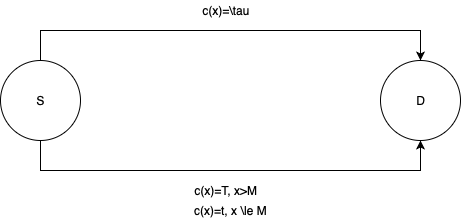
\includegraphics[scale=.7]{img/pigou}


\subsection{Парадокс Браесса}\cite[65]{gas}

\section{Трагедия общих ресурсов \footnote{англ. Tragedy of commons}}

Есть $n$ игроков, каждый из которых претендует на часть трафика $x_i\in[0,1]$.

Если общий трафик $\sum_j x_j$ превышает пропускную спопобность канала, то никто не выигрывает.
Если
$\sum_j x_j < 1$,
тогда выигрыш $u_i$ игрока 
$i$ составляет $x_i(1-\sum_j x_j)$

Найдем равновесные стратегии в этой игре.
Рассмотрим игрока $i$ и зафиксируем стратегии других игроков: $t=\sum_{j\ne i} x_j<1$.

Тогда игроку $i$ необходимо решить задачу оптимизации. 
Его выигрыш будет составлять в зависимости от $x$:
$u(i)=x(1-t-x)\to max$, который достигается при $x=(1-t)/2$.

Если все будут устремлять свой интерес к максимуму, то возникнет ситуация $\forall i: x_i=(1-\sum_{j\ne i} x_i)/2$, в силу симметричности которой $x_i=1/(n+1)$.

Эта ситуация является <<трагедией>> в силу того, что выигрыш каждого игрока мал: $u_i=1/(n+1)^2$, а сумма выигрышей всех игроков $u=n/(n+1)^2\approx 1/n$. Если ограничить общий трафик, например, $1/2$, то общий выигрыш уже будет $1/4$, что в $n/4$ раза больше\cite[5]{agt2007}.



\section{Другие подходы к проблеме}
Транспортный поток как физическая материя, состоящая из молекул \cite[168]{lukanin}
\section{Варианты практического решения}
Ценовое регулирование





\chapter{Задача о парковочных местах}

\section{Подход №1}
\setstretch{2}

Существует $M$ парковочных мест.

В игре участвуют $N$ игроков, $N >> M$.

$\tilde N$ --- количество севших за руль

$(N - \tilde N)$ --- количество поехавших общественным транспортом.

Издержки игроков $c(x)$:
\begin{itemize}
 \item  $t$, если $\tilde N\le M$,
 \item  $T$, если $\tilde N>M$;
 \item  $\tau$, альтернативный маршрут,
 \item  $t<\tau<T$
\end{itemize}

$\tau$ — альтернативный маршрут.
Сравнить его с лотереей ${t,T}$.
$P(t)$ задается $\tilde N$: $P=\frac{M}{\tilde{N}}$ (or $1$, if $M \le \tilde N$).

\textbf{Чистое равновесие}: $\frac{M}{\tilde N}t+(1-\frac{M}{\tilde{N}})T\approx\tau$.


$\tilde{N}$ (количество севших за руль) : $\frac{M}{\tilde{N}}t+(1-\frac{M}{\tilde{N}})T\le\tau$.

${N-\tilde N}$ (кто едет транспортом) : $\frac{M}{(\tilde{N}+1)}t+(1-\frac{M}{\tilde{N}+1})T\ge\tau$.

$T-\tau = \frac{M}{\tilde{N}}(T-t)$

$\tilde{N}=[\frac{M(T-t)}{T-\tau}]$ — чистое равновесие. Но «так не бывает», ибо неясно, кто эти счастливчики.

$p$ — вероятность сесть за руль.

$Q$[тебе достанется место] такова, что $\tau = Qt+(1-Q)T \Rightarrow Q(T-t)=T-\tau$, $Q*=\frac{T-\tau}{T-t}$.

Но! $Q$ должно быть вычислено как функция от $p$!

\setstretch{2.5}
$(1-p)^{N-1} + \\ (N-1)p(1-p)^{N-2} + \\ C_{N-1}^2 p^2(1-p)^{N-2} + ... + \\ C_{N-1}^{M-1}p^{M-1}(1-p)^{N-M} + \\ C_{N-1}^{M}p^M(1-p)^{N-M-1}(\frac{M}{M+1}) + \\ C_{N-1}^{M+1}p^{M+1}(1-p)^{N-M-2}(\frac{M}{M+2}) + \\ p^{N-1}\frac{M}{N} = \\ Q^*$

Решить как обратную функцию, найти $p^*$ — решение $p^*(\frac{T-\tau}{T-t})$.

\subsection{Гипотеза}
В равновесии $Np^* >> M$.

\subsection{Общее решение}

\setstretch{1}
\inputpython{../code/task1.py}{1}{41}

\subsection{Вариации}

Для $N=1000$:

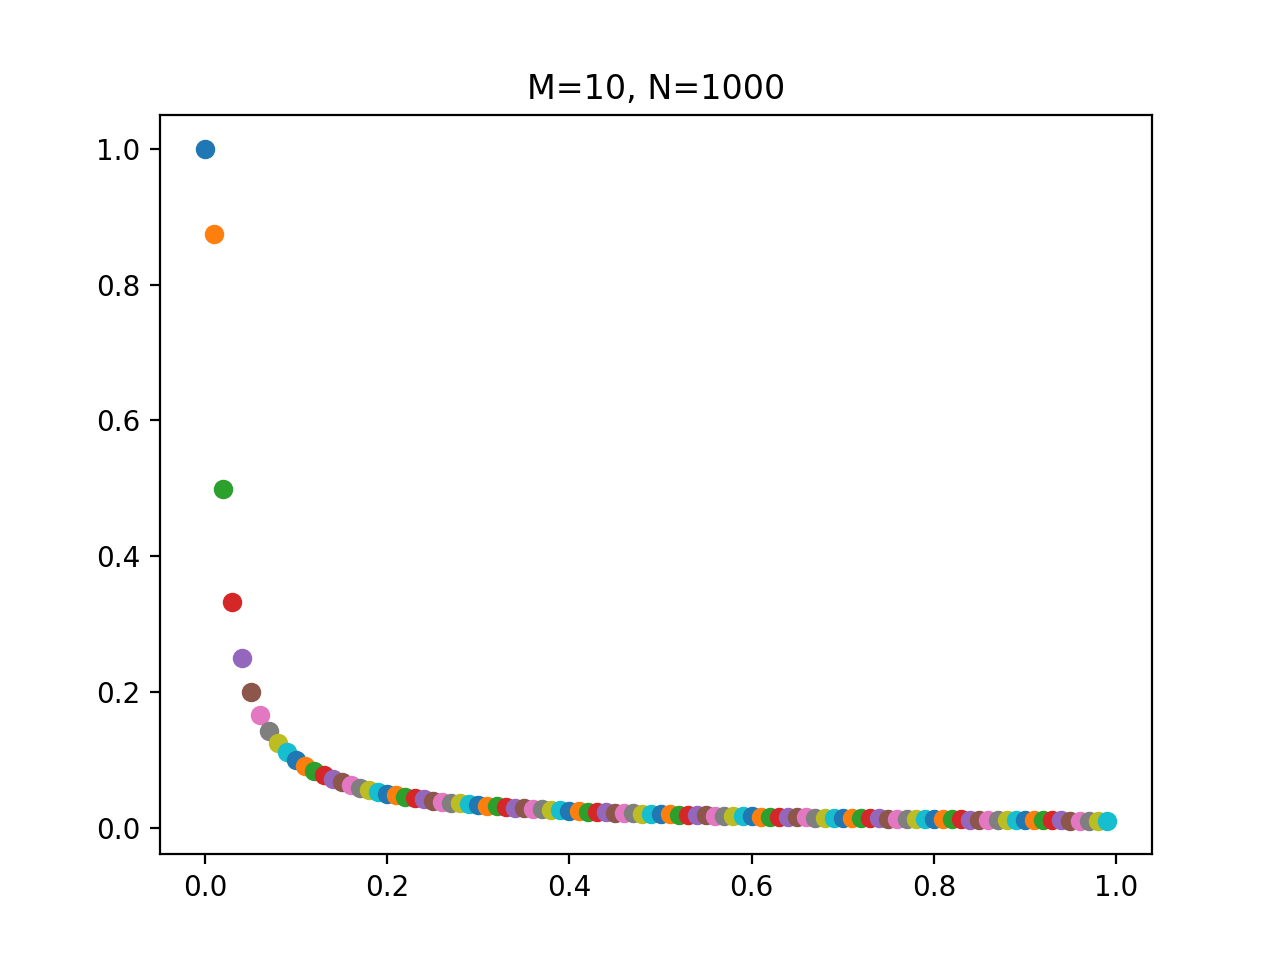
\includegraphics[scale=0.5]{img/1000_10}
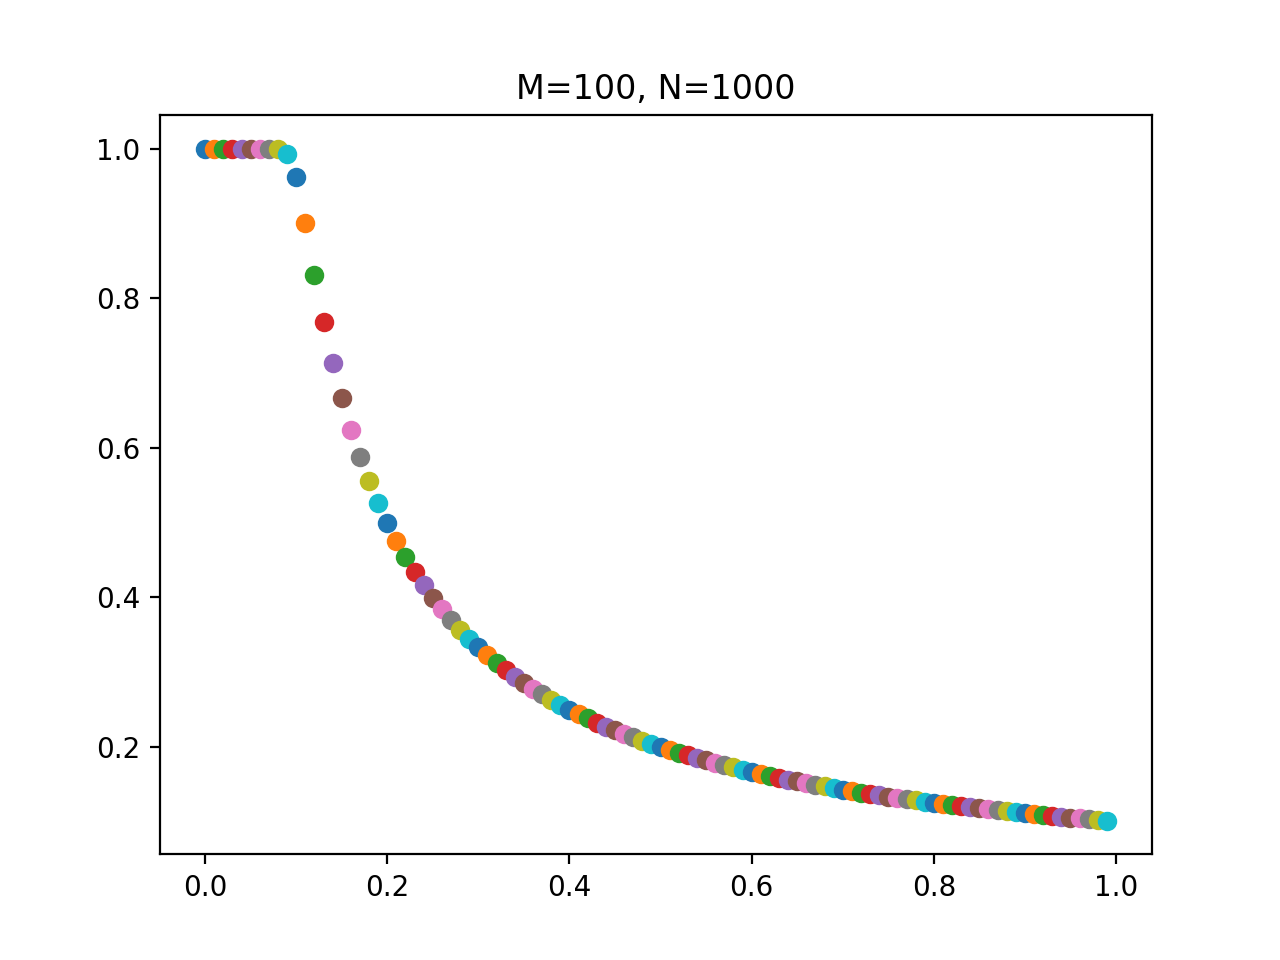
\includegraphics[scale=0.5]{img/1000_100}
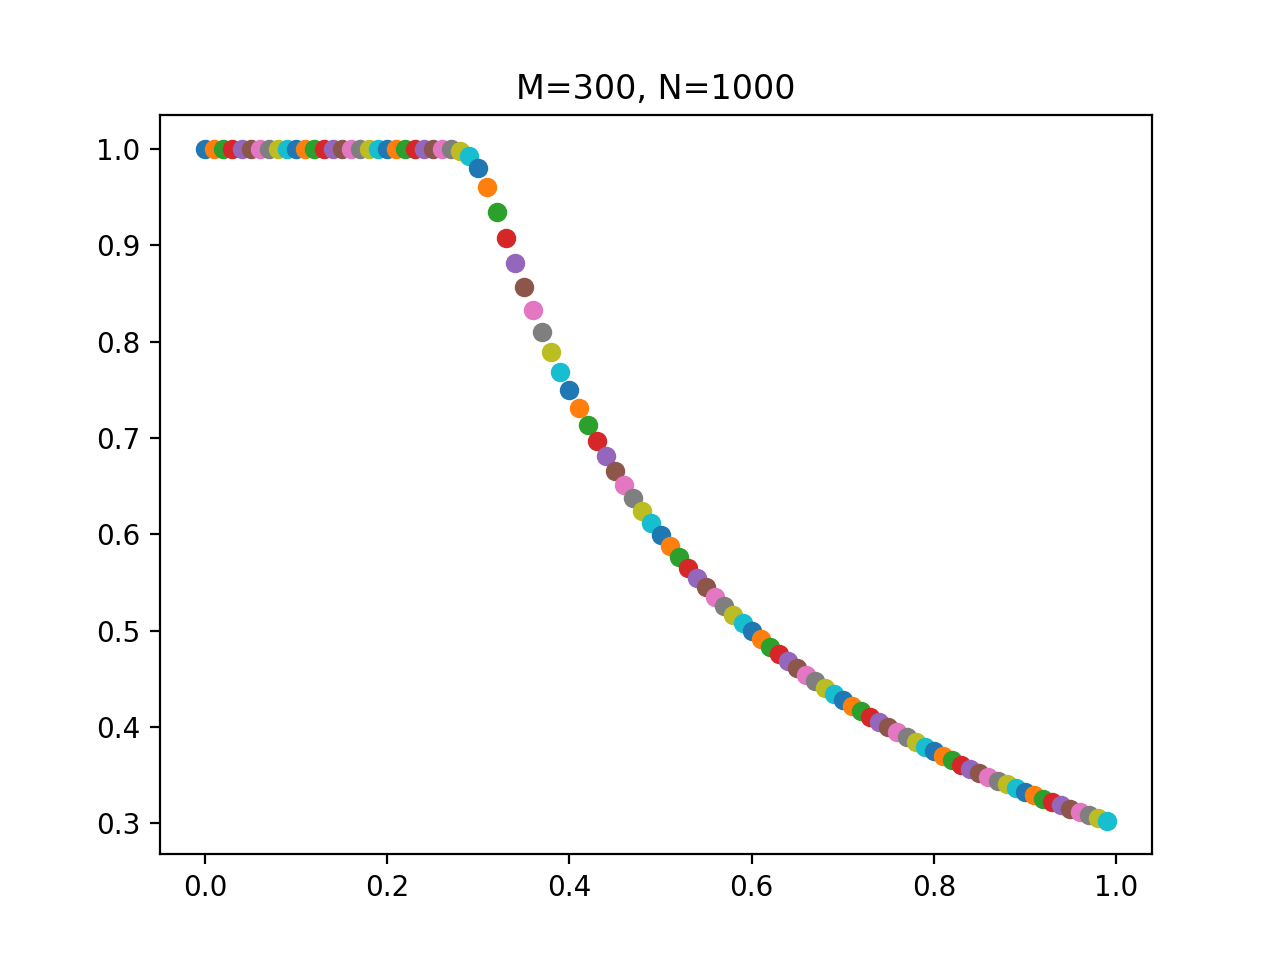
\includegraphics[scale=0.5]{img/1000_300}
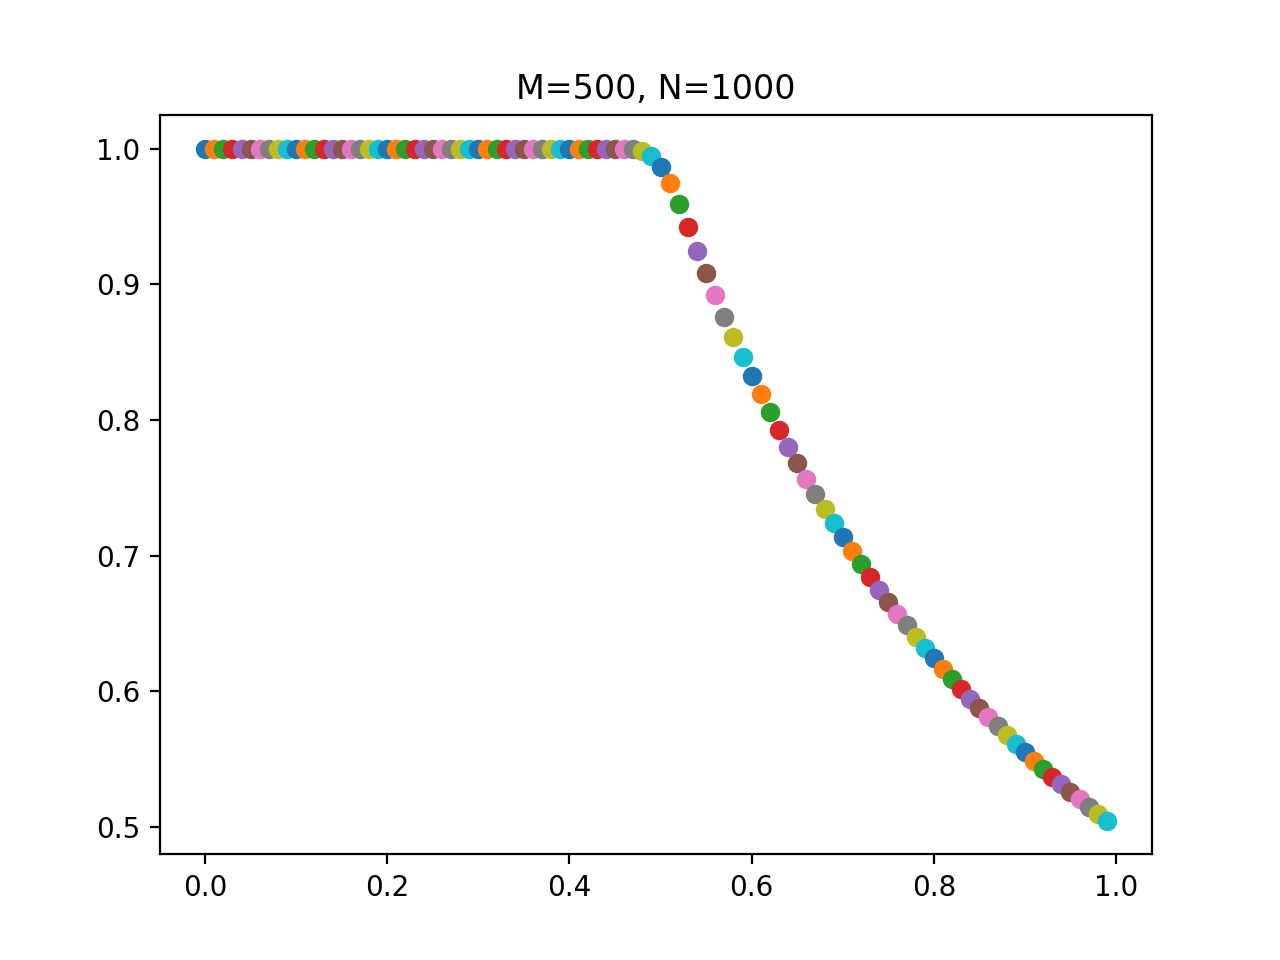
\includegraphics[scale=0.5]{img/1000_500}
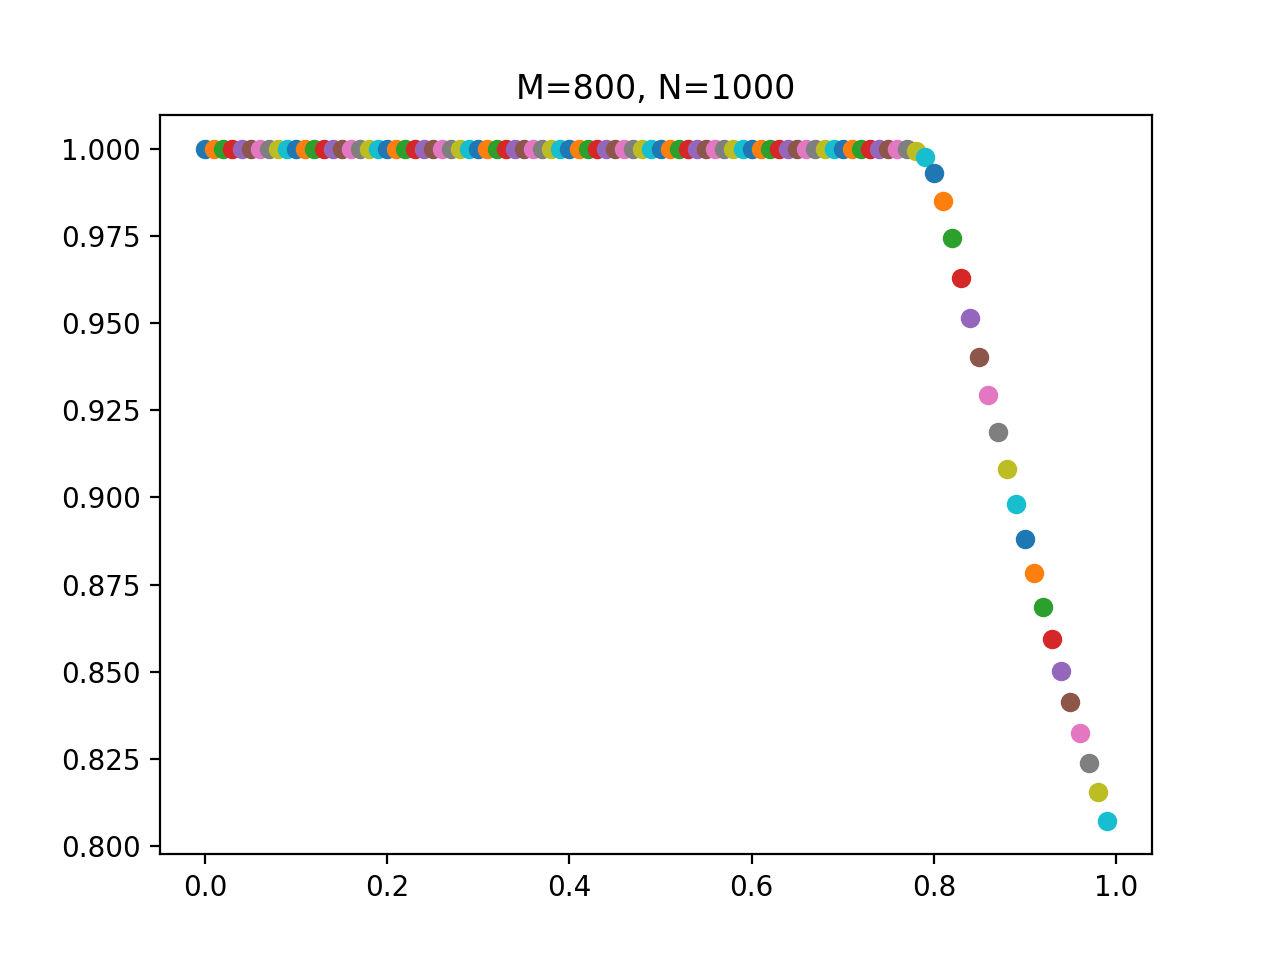
\includegraphics[scale=0.5]{img/1000_800}
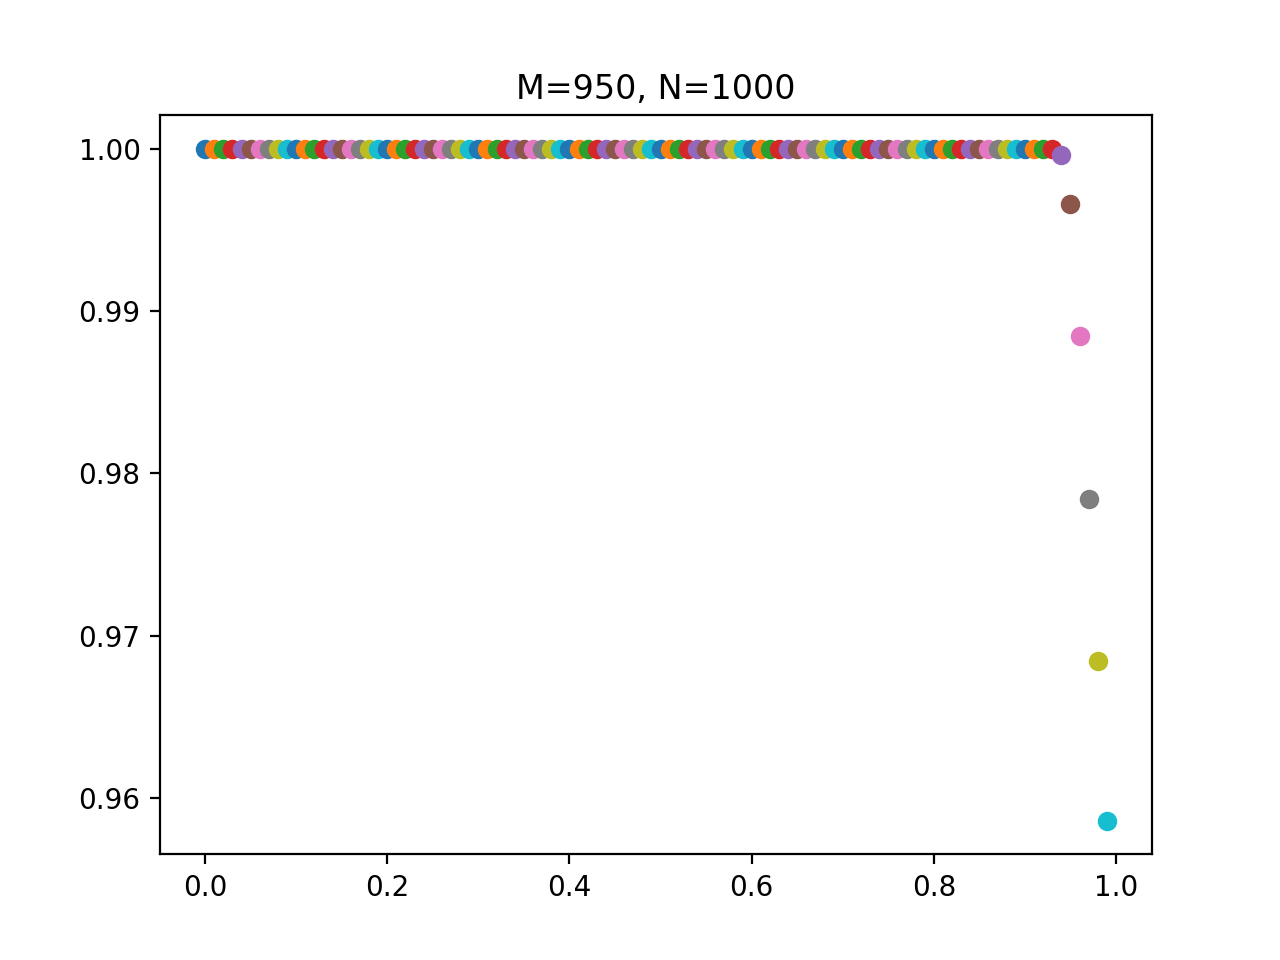
\includegraphics[scale=0.5]{img/1000_950}
\skip
Для $N=100$:

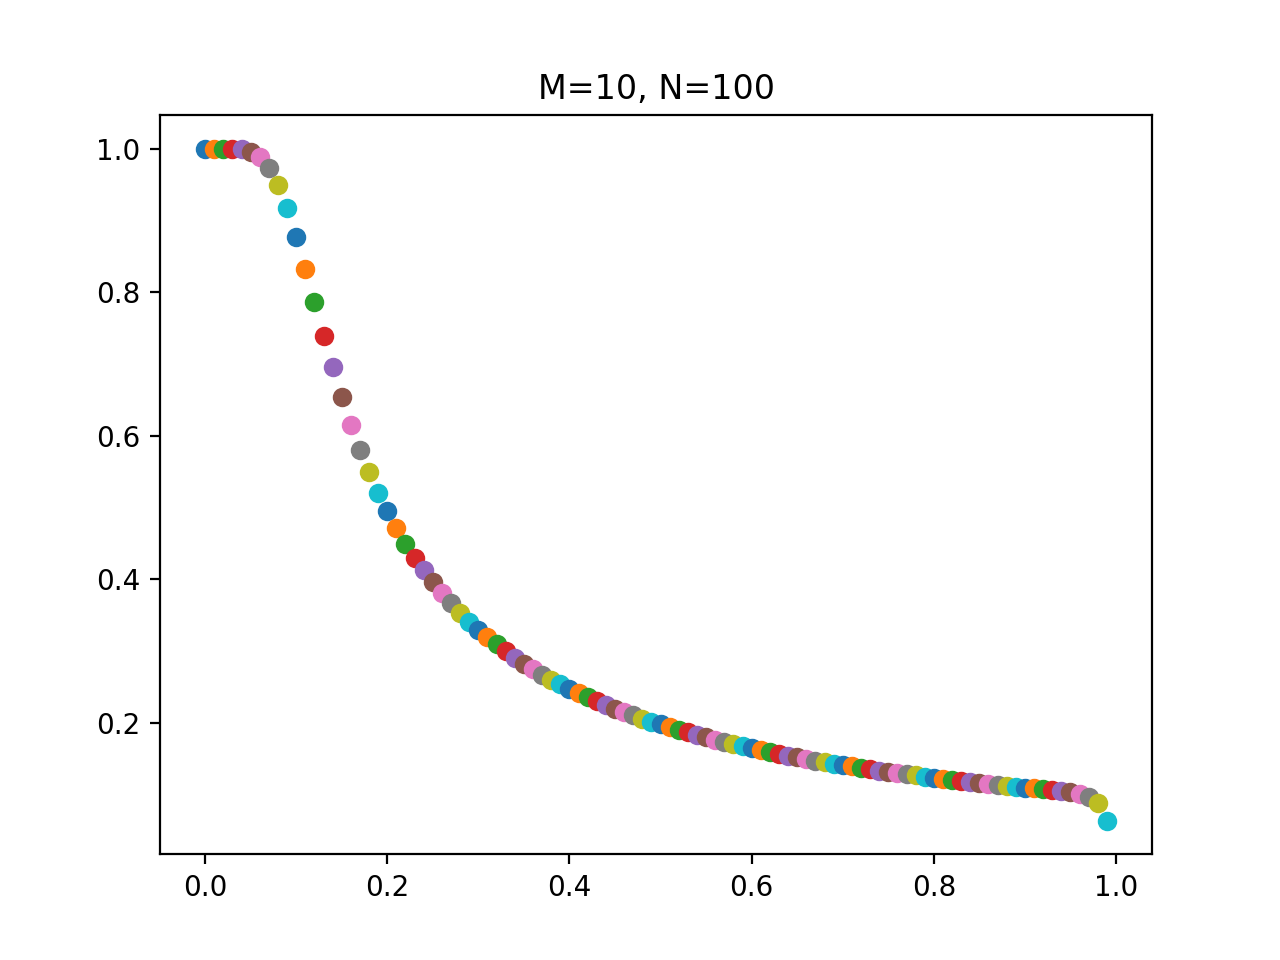
\includegraphics[scale=0.5]{img/100_10}
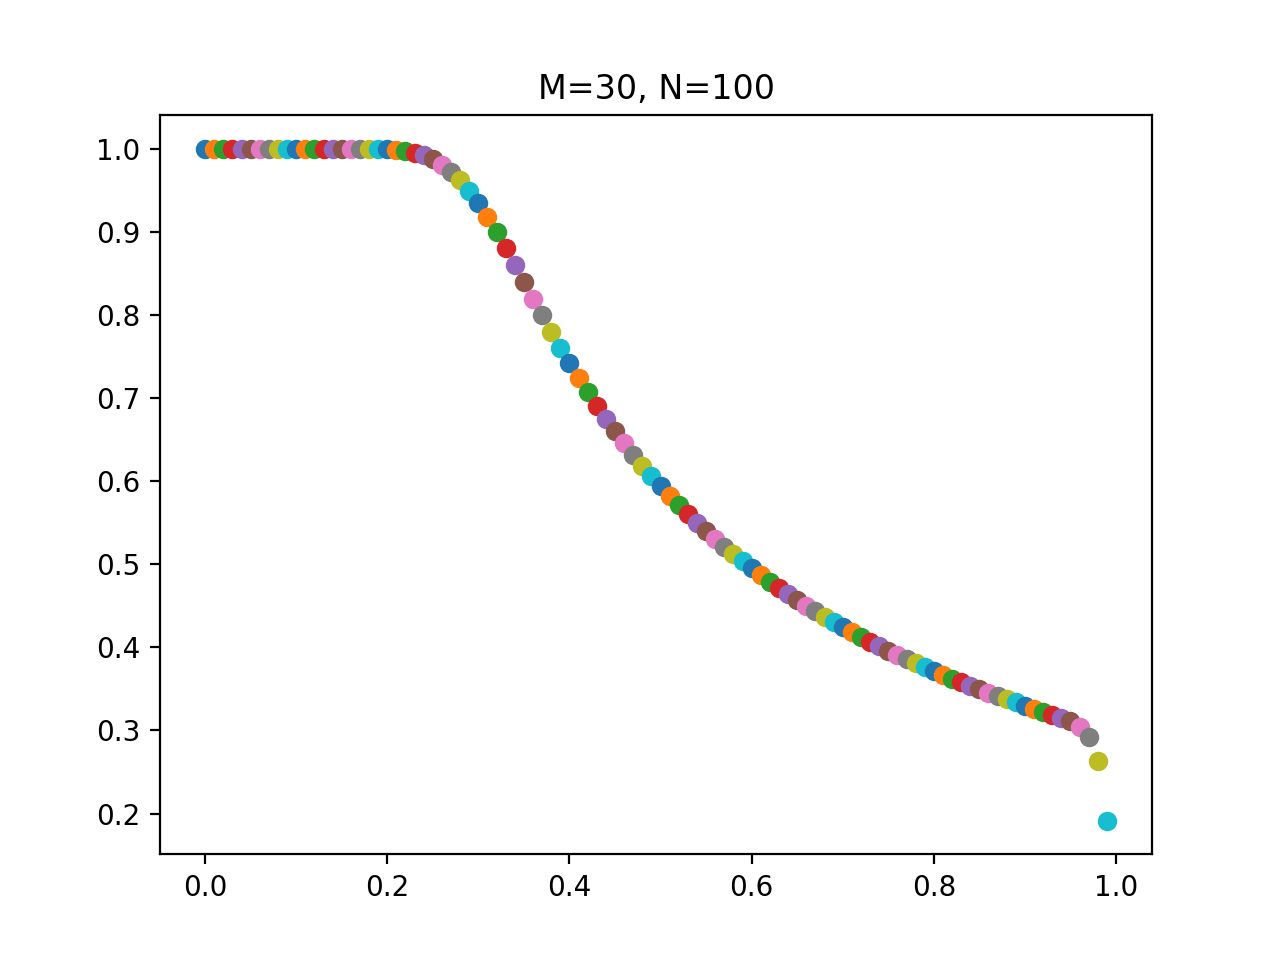
\includegraphics[scale=0.5]{img/100_30}
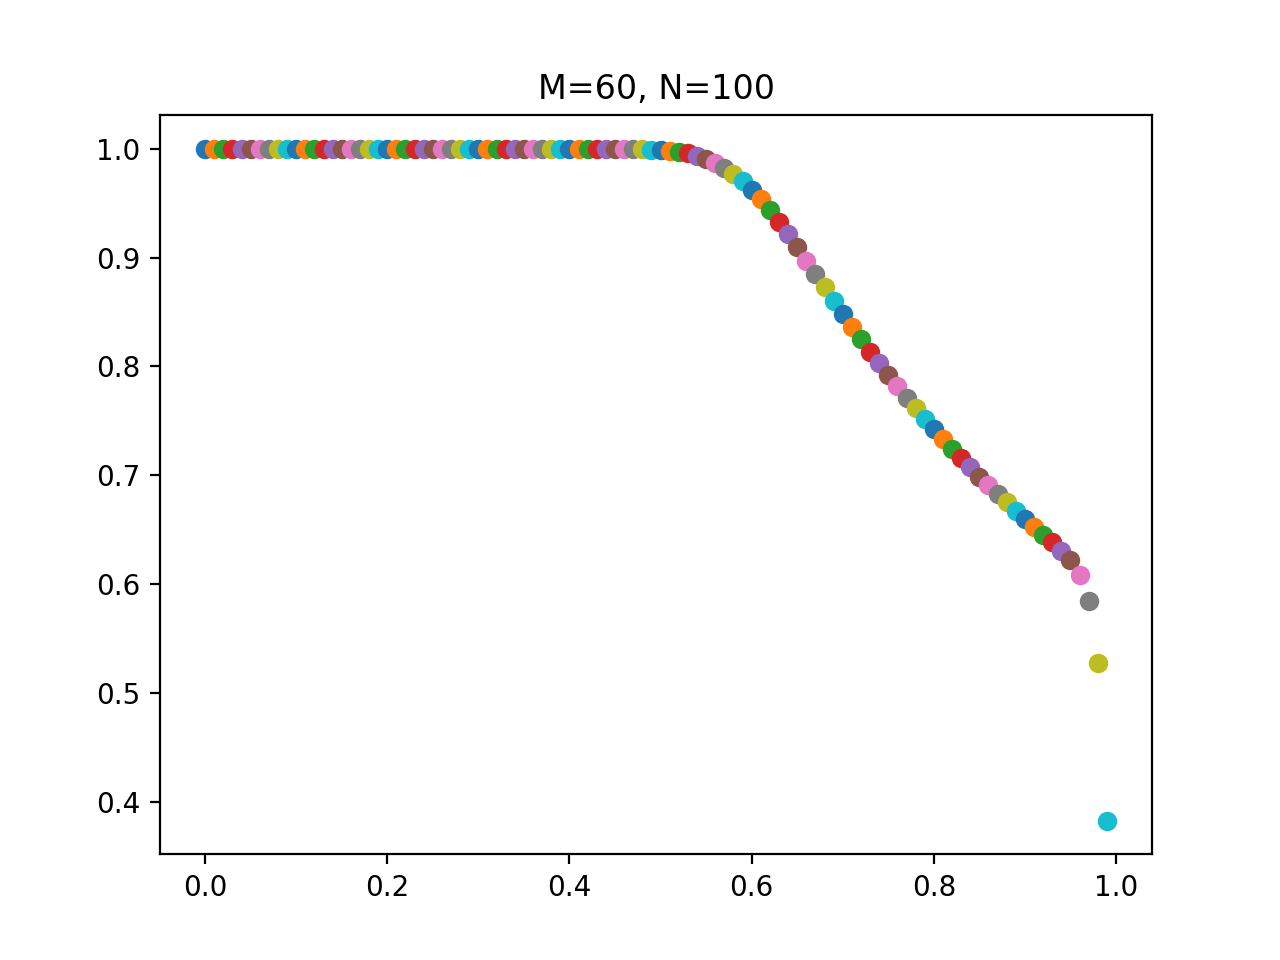
\includegraphics[scale=0.5]{img/100_60}
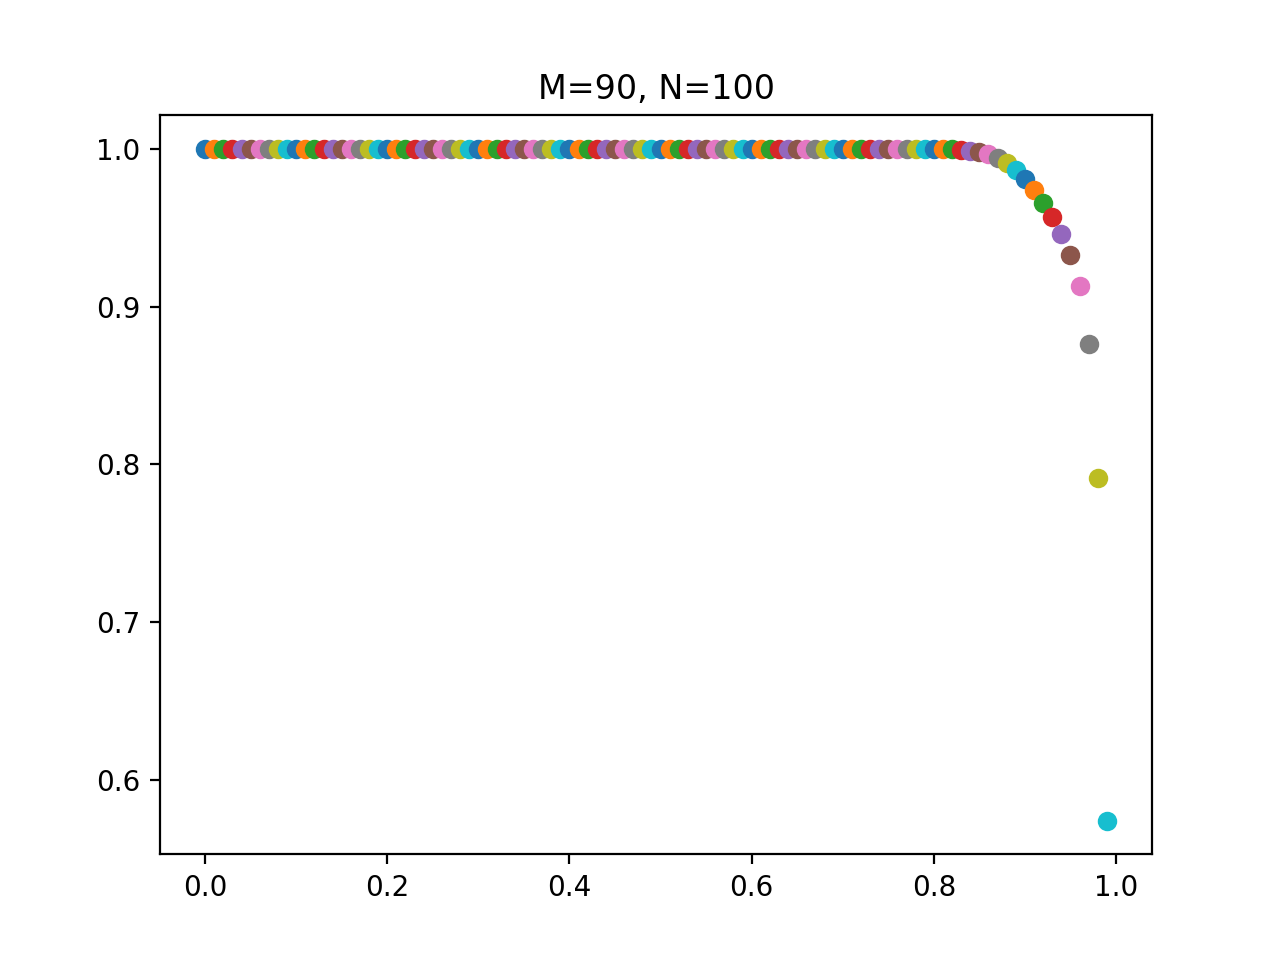
\includegraphics[scale=0.5]{img/100_90}



\section{Подход №2}

\setstretch{2}
% Это расшифровка записанного разговора

\subsection{Общая идея}

Когда M и N большие, задачу точно не нужно решать. И мы можем попробовать эту гипотезу, что не надо решать точно, проверить на таких M и N, на которых пока еще точно решается. При помощи программы решается при $M,N \le 1000$, но достаточно $M,N \le 100$. Это статфизическое приближение, которое будет простым и, скорее всего, в районе $100$ уже точным.

Если эта гипотеза верна, то для больших уже все делается приближенными вычислениями. И можно уже прилагать и проверять для примеров из раздела \ref{examples}.

Итак, есть три величины: 
\begin{itemize}
	\item $t$ --- если "повезло"
	\item $\tau$ --- если на общественном транспорте
	\item $T$ --- если попал в пробку
\end{itemize}

\begin{itemize}
	\item $M$ --- количество парковочных мест
	\item $N$ --- всего людей
\end{itemize}

Ситуация такова: мы ищем некоторое $p$ --- долю тех, кто едет (в равновесии).
Но на самом деле тогда в среднем поедет $pN$ в любом случае.
Если это большие величины, то будет очень больщая точность.
Тогда в среднем $\frac{M}{pN}$ будет вероятностью попадания, а $1 - \frac{M}{pN}$ --- непопадания (очень жесткое, грубое приближение).

И тогда получается формула $p = M/N * (T-t) / (T-\tau)$

И в равновесии отношение числа поехавших к числу парковочных мест не зависит ни от чего, кроме $T, \tau, t$: это просто $(T-t)/(T-\tau)$.

И эта гипотеза может быть проверена \textit{эмпирически}, если в данном конкретном городе разного размера стадионы дают примерно одинаковое отношение, то именно $T, \tau, t$ определяются городом, а $M$ и $N$ --- тонкости конкретных объектов проведения мероприятий.

То есть, если люди осведомлены о происходящем, то в среднем должно быть в каждом конкретном городе именно так. Это характеристика города: сколько раз происходит неудача
 % факап
 --- это первое интересное сообщение, которое можно сделать.
 % вывод, который будет очень броским

\subsection{Интересное продолжение}

$t$ и $\tau$ ни от чего не зависят.
А $T$ на самом деле зависит от $p$, и, соответственно, от величины $r= \frac{M}{pN}$.
Если много ищущих мест, то им сильно сложнее найти парковку, а если немного, то проще в соседних дворах.

% Можно протестировать какие-то очень просты формы
% Есть идея, что корень в некотором месте извлекается, потому что если территория вокруг увеличивается по квадрату, то поиск по корню. Время --- это время последующего приближения к центру после того, как ты нашел парковку
Соответственно, ключевой параметр, который нам нужен (мы его оцениваем) --- $\frac{M}{pN}$. Не само $p$, а именно выражение отношения количества парковочных мест к количеству поехавших. Это та переменная величина, которая нас и нтересует и которую мы ищем.

И в результате уравнений получается, что эта величина $r = T(r) -  \tau/(T-t)$
И теперь предполагаем, что $T = t + f(r)$, где $f(r)$ начинается с нуля при $r = 1$, а потом она растет вверх влево к бесконечности. И получается, что некоторая константа "мировая", равная $\tau - t$ --- разница между потраченным временем в транспорте и на своей машине, если ты попал сразу на парковку, приравнивается $(1-r)*f(r)$. Решение такого уравнение и есть равновесие и нужная нам величина (в равновесии эта величина будет определяться таким уравнением).

Где-то будет корень: судя по всему, она аккуратно и четко убывает от бесконечности к нулю, и где-то она пересекает в одном месте эту кривую, и дальше вопрос в \texiti{функциональной форме} $f(r)$. $f(r)$ измеряется в минутах --- это потерянные дополнительные минуты в тех же единицах, в которы измеряются $t$ и $\tau$.

Параметром является $M/N$ (вместимость парковки на вместимость зала), и $f$ будет функцией от него, соответственно, решением этого уравнения.

% Конец расшифровки записи

\subsection{Уравнения}
% Расшифровка листочка со скриншота
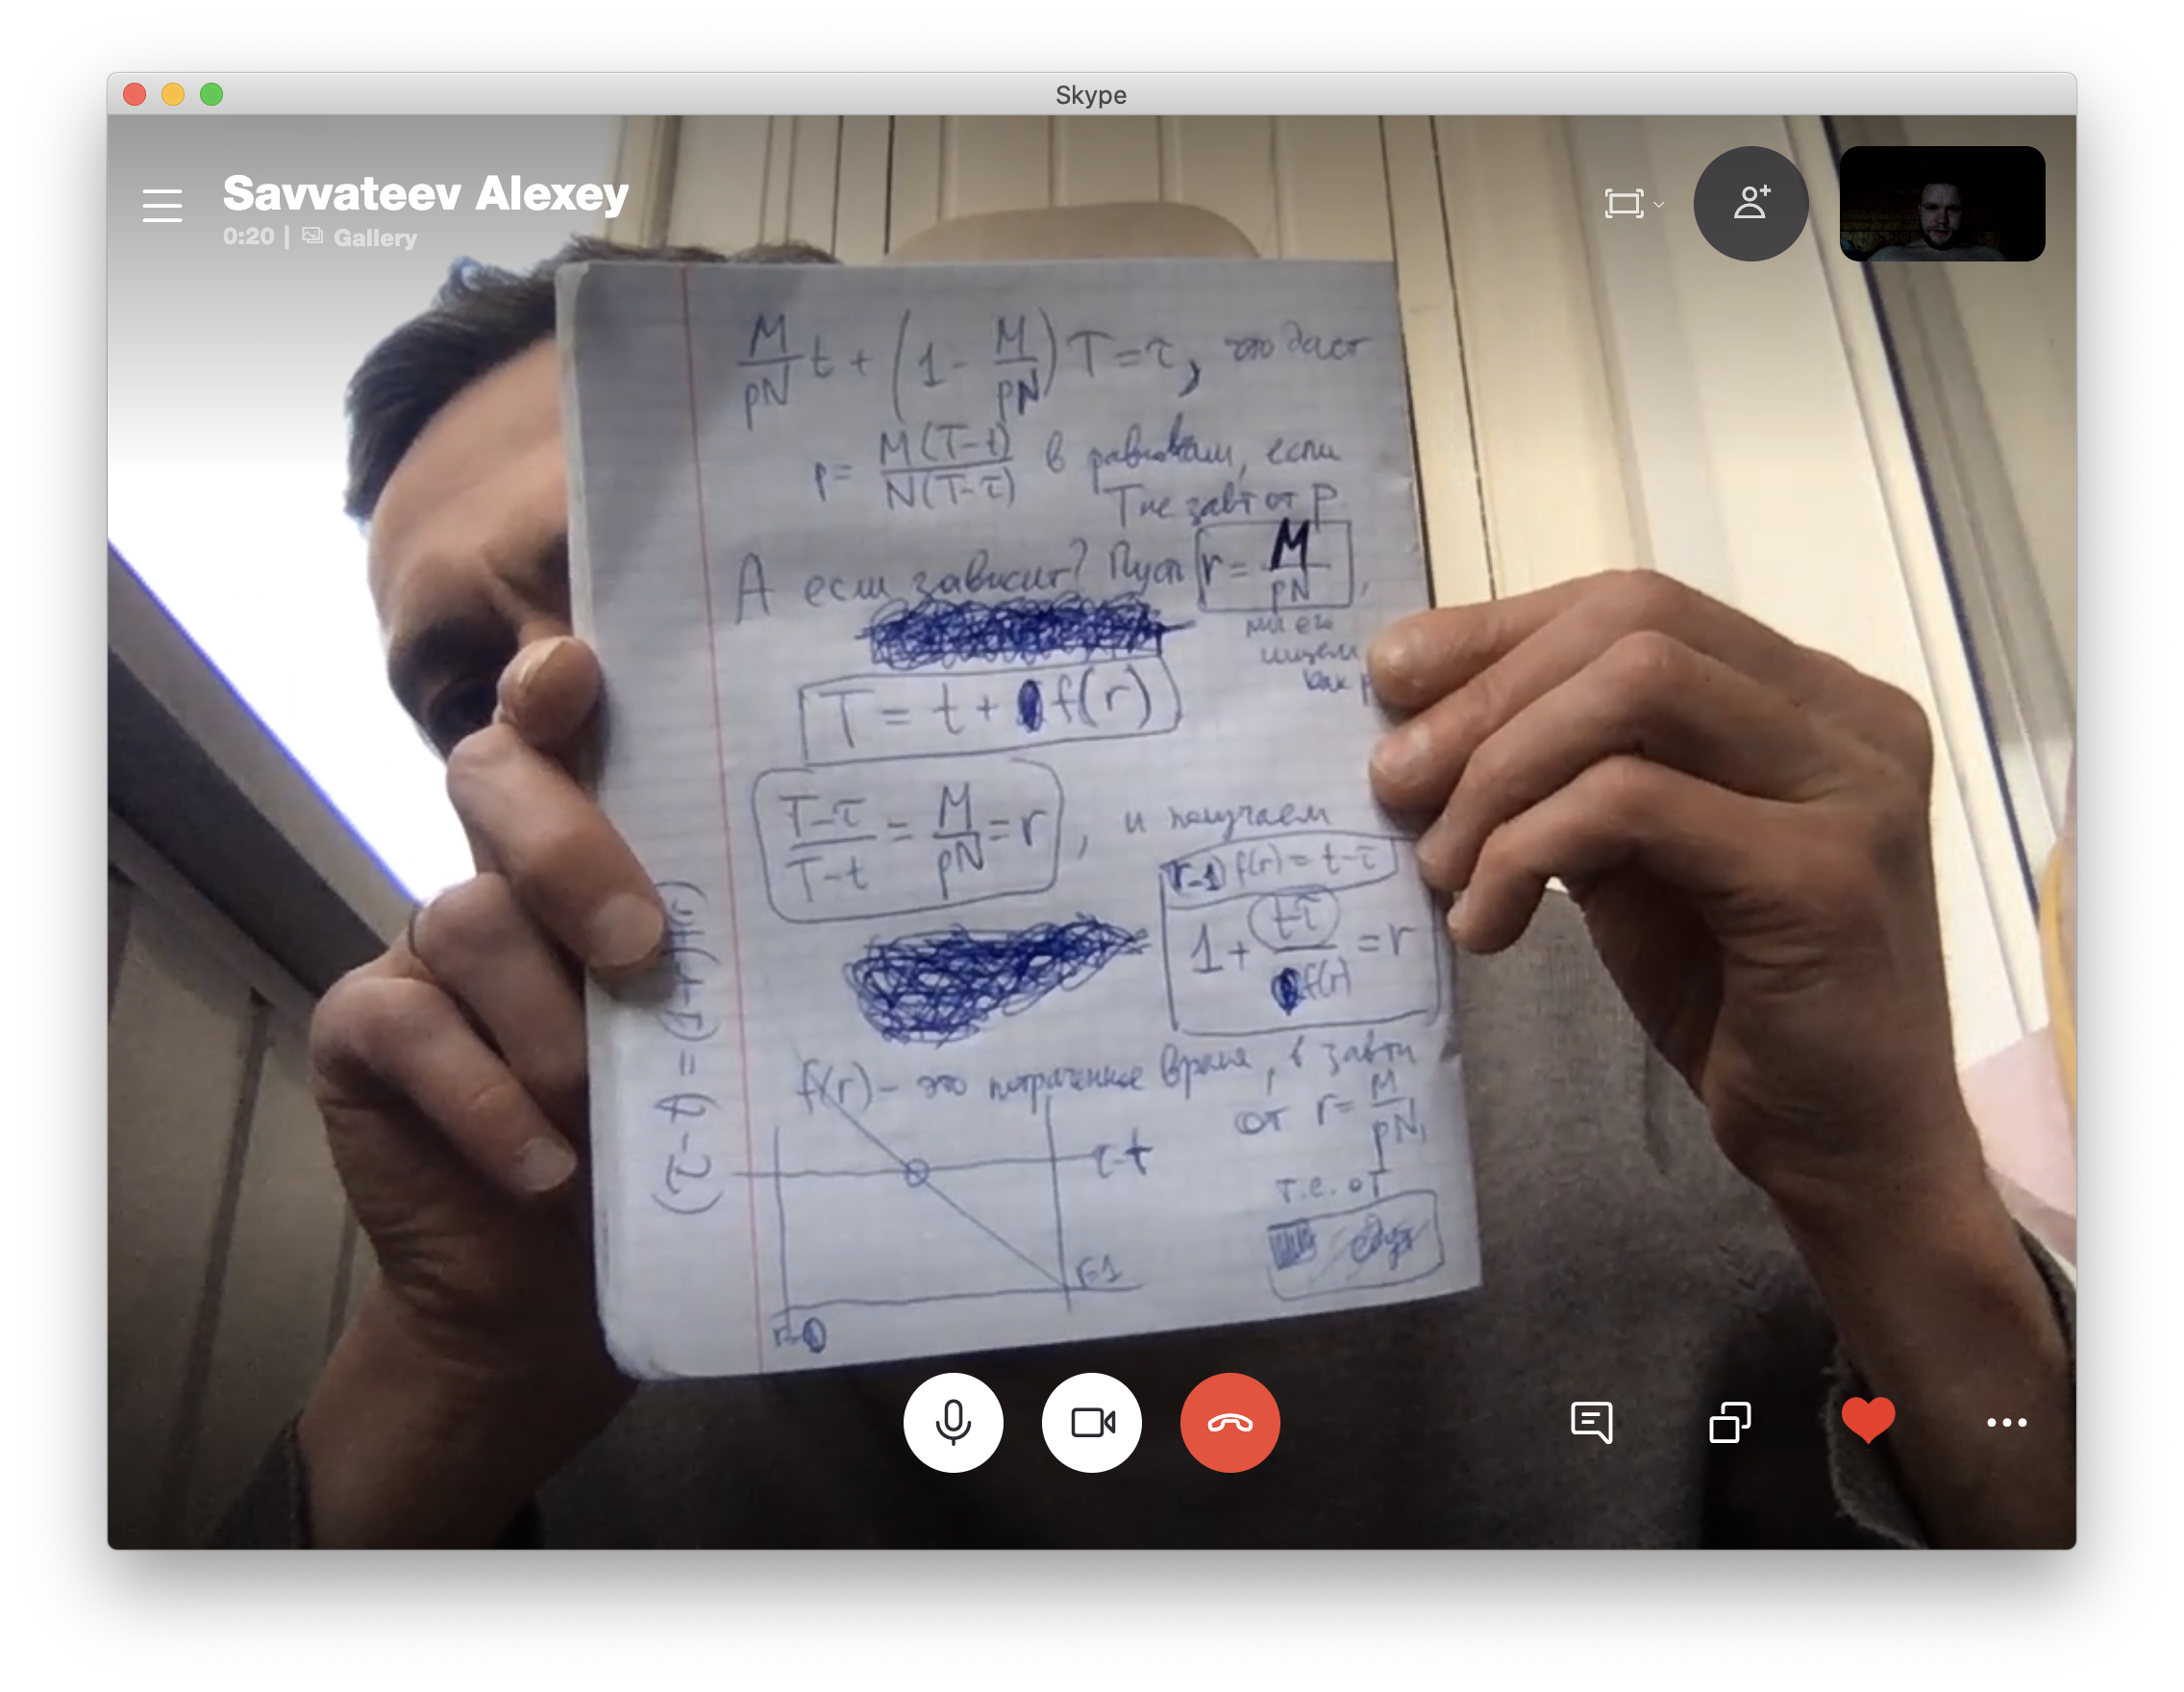
\includegraphics[scale=0.4]{img/tetrad2}
(Этот скриншот временно вместо графика)

$\frac{M}{pN} t + (1 - \frac{M}{pN}) T = \tau$,
что дает
$p=\frac{M(T-t)}{N(T-\tau)}$ в равновесии, если $T$ не зависит от $p$.

А если зависит? Пусть $r = \frac{M}{pN}$

$T = t + f(r)$

$\frac{T-\tau}{T-t} = \frac{M}{pN} = r$, и получаем $(r-1)r(r) = t - \tau$

$1 + \frac{t-\tau}{f(r)} = r$

$f(r)$ --- это потраченное время в зависимости от $r = \frac{M}{pN}$, т. е. от ...?




\setstretch{1.2}

\bigskip

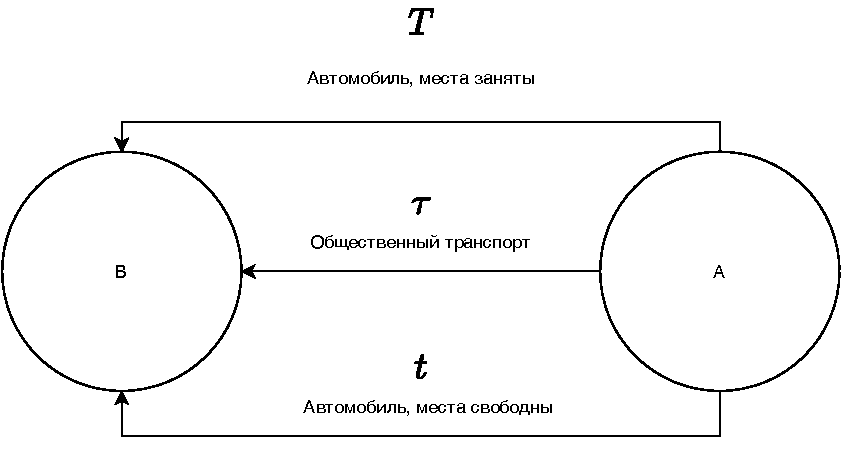
\includegraphics[scale=0.8]{img/task_scheme}


%\section{Рассуждения на тему задачи}

\section{Другие подходы к проблеме}
Транспортный поток как физическая материя, состоящая из молекул \cite[168]{lukanin}
\section{Варианты практического решения}
Ценовое регулирование

\section{Подсчет задачи на примерах из жизни}\label{examples}

Варианты с разными параметрами. Подставим некоторые реальные данные:

\subsection{СК <<Олимпийский>> (Москва)}

\begin{itemize}
	\item Количество парковочных мест: $700$ \footnote{Источник: https://carparkings.ru/parkovki/moskva/parkovka-u-sportivnogo-kompleksa-olimpijskij.html}.
	\item Максимальная вместимость: $35 000$ зрителей
	\item Максимальная вместимость после реставрации: $10 000$ \footnote{Источник: https://ru.wikipedia.org/wiki/Олимпийский}
\end{itemize}
$0,02$ в старой конфигурации
$0,07$ после реставрации

\subsection{Крокус Сити холл (Москва)}
\begin{itemize}
	\item Максимальная вместимость зала: $7233$
	\item Парковка $6000$ \footnote{Источник: https://crokus-hall.com/about/}
\end{itemize}

$0,83$

\subsection{Альберт-холл (Лондон)}

\subsection{Москва-сити}
\begin{itemize}
	\item Количество парковочных мест $10 500$  \footnote{Источник: http://moscow-city-towers.ru/parking.php}
	\item Посещаемость в день:  $175 000$ \footnote{Источник: https://moscow-city.online/news/34113/}
\end{itemize}

0,06

\subsection{Филармония (г. Майкоп)}
%\footnote{Предположим, что в Майкоп приехал Николай Басков, и все билеты раскуплены}

\begin{itemize}
	\item Мест в партере: $612$ \footnote{Источник: http://filarmoniya-ra.ru/interiors}
	\item Мест на парковке: $48$ \small{(посчитано по спутниковой карте)}
\end{itemize}
\begin{figure}
	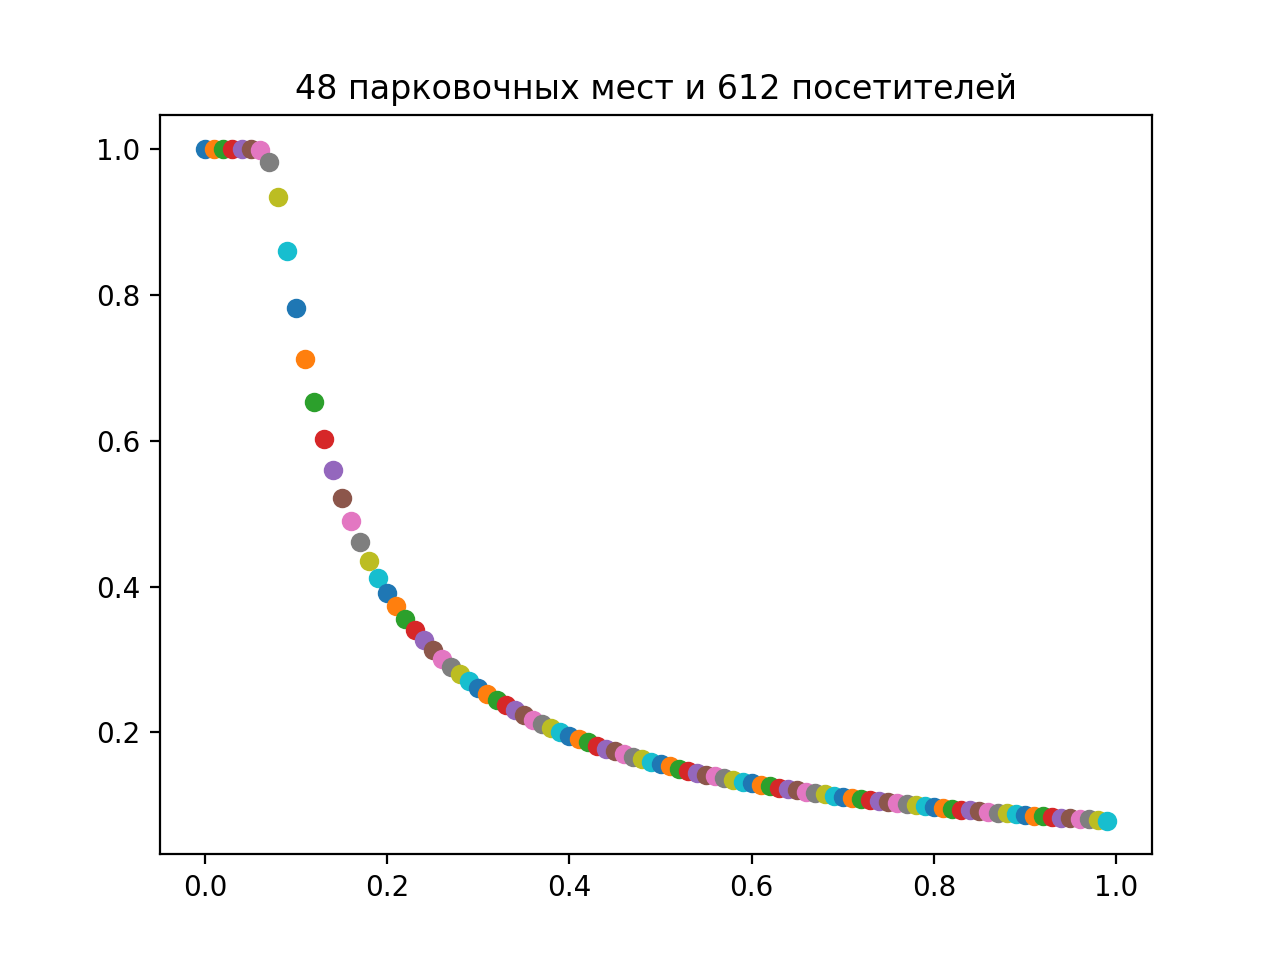
\includegraphics[scale=0.6]{img/612_48}	
\end{figure}

\begin{figure}
	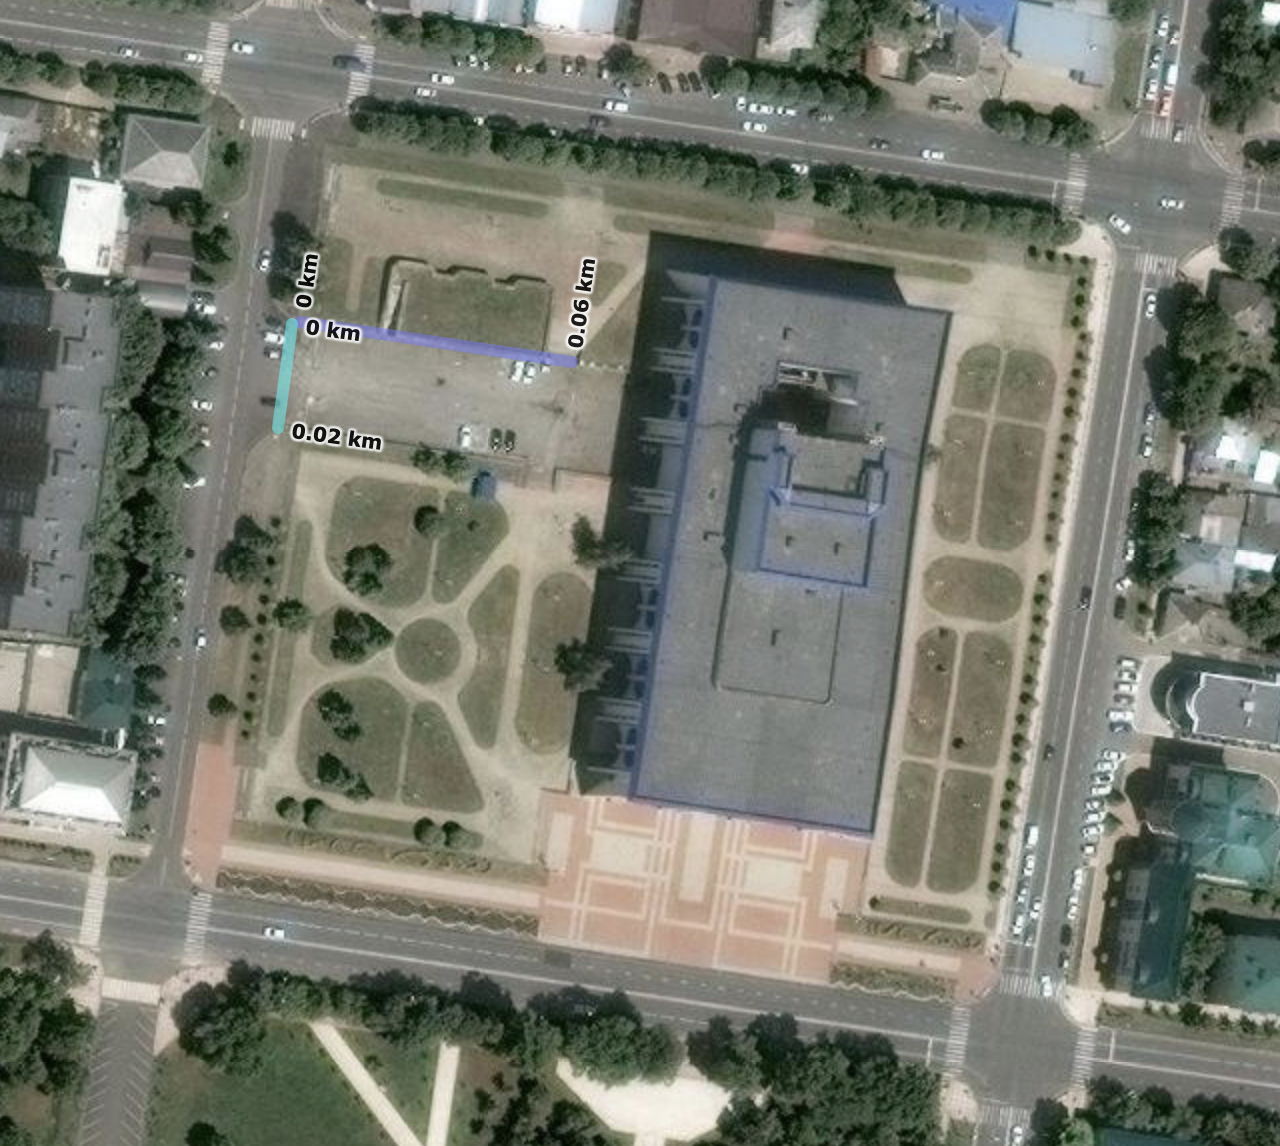
\includegraphics[scale=0.3]{img/filarmony_parking}
	\caption{Майкопская филармония на спутниковых Яндекс-картах}
\end{figure}

0,07


\chapter{Выводы исследования}

\begin{itemize}
\item Разработана модель ...
\item В процессе анализа...
\item В ходе ...
\end{itemize}
% Давно известно, что...
% Анализ, проведенный в гл... показывает, что ...
% Прикладная задача
% Решение прикладной задачи методами программмирования
% Применение в жизни
% Коммерческое применение...
% И, наконец, последний вывод...


\chapter{Приложения}
\section{Основные концепции теории
игр
\footnote{
По сути, приложение является переводом главы из \cite{Association:2018aa}
}
}

%Сон Ук Ким Университет Соган, Южная Корея

%\emph{Переведено Егором Кузьмичевым 13 мая 2020 года}

\subsection{Краткое
описание}

Теория игр по-разному описывается как наука о стратегии или наука о
разрешении конфликтов. В ее основе лежат характеристики математической
конструкции: четкий набор концепций и положений, фундаментальные теоремы
и их применение к проблемам реального мира. Тот факт, что
рассматриваемые вопросы в основном относятся к областям социальных наук,
ставит, однако, теорию игр в особое положение по сравнению с другими
математическими и научными дисциплинами. Вслед за книгой фон Неймана и
Моргенштерна принято анализировать то, что мы называем игровыми
ситуациями, используя уже существующие или специально созданные для этой
цели салонные игры - как аналитические модели. Что и делается в этой
главе.

\subsection{Введение}

За последнее десятилетие возник широкий интерес к вопросам, которые
находятся на пересечении сетевого дизайна и теории игр. В последнее
время алгоритмическая теория игр является одной из наиболее заметных
областей роста в теоретической информатике и телекоммуникациях
\cite{Wooldridge:2012}. Теория игр - это математическая теория
взаимодействия между рациональными агентами. В частности, она
фокусируется на принятии решений в ситуациях, когда решение каждого
игрока может повлиять на результаты других игроков. В таких ситуациях
каждый игрок должен учитывать, как будут действовать друг с другом
игроки, чтобы сделать оптимальный выбор. В теории игры под ``игрой''
понимается абстрактная математическая модель многих агентов, принимающих
рациональные решения \cite{Wooldridge:2012}. В теории игр моделируемая
ситуация определяется как игра, предсказывающая исход сложных
взаимосвязей между сущностями. Обычно нормальная игровая форма (\(G\))
может быть сформулирована тремя составляющими: игроки, стратегия или
пространство действий для каждого игрока (т. е. набор стратегий) и
последствия действий (т. е. набор выплат или выигрышей). Математически
\(G\) определяется как
\(N\in \{N, \{S_i\}_{i\in N}, \{u_i\}_{i\in N}\}\).

\begin{itemize}
\item
  \(N\) - это конечный набор игроков.
\item
  \(S_i\) - это набор стратегий с игроком i.
\item
  Функция полезности игрока \(i\) (\(u_i\)) может быть представлена как
  степень удовлетворенности, полученная игроком \(i\), как функция
  выбранной им стратегии, \(s_i\), так и действие других игроков:
  \(s_{-i} = (s_1,....,s_{i-1}, s_{i+1},...,s_N)\).
\end{itemize}

Игроки - это лица, принимающие решения, о том, как они действуют. Игрок,
например, компания, нация, беспроводной сетевой узел или даже
биологический вид, может быть независимым и должен совершать конкретные
действия, которые имеют взаимные, возможно, конфликтующие друг с другом
последствия. Обычно предполагается, что игроки индивидуально
рациональны, действуют рационально и стараются обеспечить наилучший
возможный итог игры в соответствии со своими предпочтениями. Набор
стратегий представляет собой набор различных действий, доступных игроку.
Каждый игрок имеет ряд возможных действий и может выбрать действие,
определяющее конечный результат игры. Любое действие игрока должно быть
выражено соответствующей функцией полезности, которая сопоставляет
каждое действие с реальным числом. Функция выигрыша (или полезности)
количественно определяет удовлетворение, которое игрок может получить от
определенного действия. Обычно полезность игрока соответствует
полученной выплате за вычетом понесенных расходов. На основании
полученных выплат можно оценить результат для разных игроков. Поэтому
индивидуумы, принимающие решения (т.е. игроки), стараются найти лучшие
действия.

Наиболее классическим примером теории игры является ``Дилемма
заключенного'' (``Prisoner's dilemma,'' n.d.). Дилемма заключенного -
это канонический пример игры, анализируемый в теории игр, который
показывает, почему два индивидуума могут не сотрудничать, даже если
кажется, что это в их интересах. Проще говоря, двум заключенным
предъявляются обвинения в преступлении, которое они, скорее всего,
совершили вместе, но полиция не уверена в этом. Таким образом, они
заключают сделку, в рамках которой допрашивают каждого подозреваемого в
частном порядке, и могут по своему выбору ``сотрудничать'' (т.е.
утверждать, что они не совершали преступления) или ``предавать'' (т.е.
признаваться в совершении преступления). Наказания являются следующими:

\begin{enumerate}
\item
  Если один заключенный ``сотрудничает'', а другой ``предаёт'', то
  ``предатель'' освобождается, а ``кооператор'' должен провести в тюрьме
  десять лет.
\item
  Если оба заключенных сотрудничают, полиция не хочет рисковать жизнью
  двух невиновных, поэтому дает год тюрьмы каждому.
\item
  Если оба заключённых ``предадут'' друг друга, они будут наказаны за
  своё преступление трёхлетним сроком.
\end{enumerate}

Если другой заключенный решает сотрудничать, то предательство выгоднее,
а если другой заключенный решает предать, то предательство тоже
выгоднее. Поскольку предательство всегда вознаграждается больше, чем
сотрудничество, то все чисто рационально мыслящие заключенные предадут
друг друга. Поэтому в классическом варианте игры над сотрудничеством
доминирует предательство. Интересная часть этого результата заключается
в том, что стремление к индивидуальному вознаграждению логически
приводит заключенных к предательству обоих, даже если бы они получили
лучшее вознаграждение, если бы оба сотрудничали.В этой ситуации
единственным рациональным выбором для заключенного, минимизирующего
наказание, является предательство, так как это дает ему лучший
результат, что бы ни делал другой. Следовательно, и то, и другое хуже,
если они оба рациональны, чем если бы оба были иррациональны. В
частности, каждый человек получает более легкое наказание, если оба
пытаются максимизировать свое наказание, чем если оба пытаются его
минимизировать. Это так называемая ``дилемма заключенного''.

Теоретико-игровые дилеммы не просто любопытны, они возникают на
протяжении всей социальной жизни. Поэтому концепция дилеммы заключенного
используется в таких социальных науках, как экономика, политика и
социология, а также в биологических науках, таких как этика и
эволюционная биология \cite{Howard:1971}. Гонки вооружений в период холодной
войны могут быть смоделированы как ситуация ``дилеммы заключенного''.
Хотя наилучшая стратегия заключается в разоружении западной и восточной
сторон, рациональным курсом для обеих сторон является вооружение. Это
действительно то, что произошло в реальном мире, и обе стороны вложили
огромные ресурсы в военные исследования и вооружение.

Первоначально теория игр предполагает, что игры представлены в
нормальной форме, в виде матрицы или дерева. Она также предполагает, что
игроки не имеют ограничений по вычислительным ресурсам, так что они
могут хранить в памяти все дерево игры, и могут просчитать все возможные
последствия каждого хода. Учитывая эти допущения, и до тех пор, пока мы
сможем представить алгоритм, который будет хорошо играть в игру за
конечное время, игра будет, по сути, тривиальной. Это означает, что
конечная игра для двух игроков с совершенной информацией (например, в
шахматы) считается тривиальной. Однако, принимая во внимание
ограниченность ресурсов игроков, становится очевидным, что игрок никогда
не сможет сохранить в памяти (для большой партии) всё дерево игры, а
также не учтет все возможные последствия каждого действия. Таким
образом, игрок должен выборочно рассматривать возможности и результаты и
принимать решения, основываясь на менее совершенной информации.
Поскольку игрок вообще не может видеть точного влияния хода на конечные
цели игры, из этого следует, что его рассуждения должны быть
эвристическими \cite{Pell:1993}.

Обучение можно определить как способность принимать разумные решения,
самостоятельно адаптируясь к динамике окружающей среды, учитывая опыт,
накопленный в прошлых и настоящих состояниях системы, и используя
долгосрочные оценки выигрышей. Обучение всегда зависит от объема
информации, доступной каждому игроку. В результате, изучение
алгоритмической теории игр в последние годы становится все более важной
частью алгоритмических исследований.В частности, машинное обучение
достигло постоянного прогресса в разработке методов, которые могут
обобщать данные, адаптироваться к изменяющимся условиям и улучшать
производительность с помощью опыта, а также прогресса в понимании
фундаментальных проблем, лежащих в основе. В последнее время растет
интерес к исследованиям на стыке теории игр и алгоритмов обучения. Такая
работа мотивирована наблюдением, что хотя эти две области традиционно
рассматривались как разрозненные области исследований, на самом деле
между ними существует большая общность, которая может быть использована
в рамках обеих областей. Благодаря интеграции по распределению стратегий
противника, а не простому эмпирическому усреднению, последние
исследования показывают, как идеи теории игр могут быть использованы для
получения новых алгоритмов обучения \cite{Blum:2008}.

Большинство общучающих алгоритмов предназначены для улучшения программы,
на основании наблюдений или игры против умелых соперников. Хотя,
безусловно, важно понимать, как программа (или игрок) может учиться у
хороших игроков, не менее важно знать, как эти игроки стали такими
хорошими . Гораздо меньшая часть работы по обучению рассматривала, как
программы могут стать сильными игроками, не полагаясь при этом ни на
глубокий анализ, ни на опыт взаимодействия с экспертами. Большинство из
этих подходов можно рассматривать как самостоятельную игру, в которой
либо один игрок, либо целая группа игроков развивается во время
соревнований на большом количестве конкурсов. Связанная с этим методика,
которую также можно рассматривать как форму самостоятельной игры,
заключается в том, что базовая игровая программа научилась предсказывать
ожидаемый результат позиции, если в нее играют случайные игроки. Это
оказалось эффективным при построении оценочных функций для некоторых игр
\cite{Pell:1993}.

Для интерпретации теории игр существуют описательные и нормативные
интерпретации. Эти две интерпретации представляют очень разные критерии
для вопроса о том, применима ли теория игр \cite{Wooldridge:2012}. В рамках
описательной интерпретации мы можем рассматривать теорию игр как попытку
предсказать, как будут вести себя игроки в стратегических ситуациях.
Поэтому описательная интерпретация предполагает, что мы должны искать,
успешно ли теория игр предсказывает, как люди будут делать выбор в
ситуациях, которые мы можем смоделировать как игры. Некоторые ученые
полагают, что, найдя равновесие игр, они могут предсказать, как будут
вести себя реальные человеческие группы при столкновении с ситуациями,
аналогичными изучаемой игре. Эта описательная интерпретация теории игр
подверглась недавней критике. Теоретики игры предполагают, что игроки
являются Homo economicus и всегда действуют рационально, чтобы
максимизировать свою выгоду (``Homo economicus'', n.d.). Более того, они
реагируют, сравнивая свои предположения с предположениями, используемыми
в физике. Таким образом, хотя их предположения не всегда совпадают, они
могут относиться к теории игр как к разумному научному идеалу, сходному
с теми моделями, которые используются физиками. Однако реальные игроки в
игры, например, люди, часто действуют либо иррационально, либо не играют
в стратегии равновесия. Поэтому основополагающие допущения, выдвигаемые
теоретиками игры, часто нарушаются, и вопрос о том, как игроки достигают
равновесия, остается открытым. В соответствии с нормативной
интерпретацией мы можем рассматривать теорию игры как предписывающий
направление действий игроков. То есть теория игр рассказывает игрокам о
том, как они должны действовать. Поэтому нормативная интерпретация
предполагает, что мы должны изучить, можем ли мы получить результаты,
которые лучше, чем те, которые мы могли бы получить в противном случае
\cite{Wooldridge:2012}. Некоторые ученые, придерживающиеся нормативного
взгляда, рассматривают теорию игр не как инструмент прогнозирования
поведения людей, а как предложение о том, как люди должны себя вести.
Поскольку равновесие Нэша в игре представляет собой лучший ответ на
действия других игроков, игра в стратегию, которая является частью
равновесия Нэша, кажется уместной. Однако эта нормативная интерпретация
теории игр также подверглась критике. Во-первых, в некоторых случаях
уместно играть в стратегию, не являющуюся частью Нэшевского равновесия,
если один из них ожидает, что другие тоже будут играть в стратегию, не
являющуюся частью Нэшевского равновесия. Во-вторых, в некоторых случаях,
например, в ``Дилемме заключенного'', каждый игрок, преследующий свои
собственные интересы, приводит всех игроков в худшее положение, чем если
бы они не преследовали свои собственные интересы. Некоторые ученые
считают, что это свидетельствует о провале теории игр как рекомендации к
правильному действию.

\subsection{Классификация игр}

Игры могут быть классифицированы по определенным значимым признакам и
свойствам. Обычно игры можно разделить на две различные группы по
различным двоичным критериям: является ли игра симметричной или нет,
является ли игра статичной или нет, содержит ли игра совершенную
информацию или несовершенную информацию и так далее.В данном подразделе
мы изучаем, как классифицировать игры (``Game theory'', n.d.).

\subsubsection{Некооперативные игры vs.~кооперативные игры}

Как правило, игры можно разделить на некооперативные и кооперативные,
независимо от того, являются ли игроки кооперативными или
некооперативными. Игра является некооперативной, если игроки принимают
решения самостоятельно и не могут сформировать обязательные для
исполнения обязательства. Поэтому игроки находятся в конфликте и не
общаются и не сотрудничают друг с другом. Поэтому игроки стараются
обеспечить наилучший возможный исход в соответствии с функцией
полезности. Дилемма заключенного и битва полов - это хорошо известные
некооперативные игры.

Кооперативные игры, также называемые коалиционными играми, - это игры, в
которых игроки берут на себя обязательные обязательства и находят
полезным сотрудничество в игре. Поэтому для выполнения обещаний игроков
необходимы правовые системы или строгие правила. В кооперативных играх
анализируются совместные действия групп, т.е. каков результат, если
группа игроков сотрудничает. Поэтому основной интерес в кооперативных
играх заключается в справедливом распределении результата между каждым
игроком в соответствии с его вкладом. В кооперативных играх это
невозможно. Вектор Шэпли и решение Нэша задачи о сделках (в литературе
часто используется аббревиатура NBS, от англ. Nash bargaining solution
--- решение Нэша для переговоров) - это хорошо известные кооперативные
игры.

Однако эта двоичная классификация была поставлена под сомнение. Поэтому
значительные усилия были приложены к тому, чтобы связать два типа
игровых моделей. Недавно были предложены гибридные игры в
полукооперационной манере. Эти игры содержат кооперативные и
некооперативные элементы. Например, в кооперативной игре формируются
коалиции игроков, но они играют некооперативно.

\subsubsection{Статические игры vs.~Динамические игры}

Статические игры также называют стратегическими, односерийными,
одноступенчатыми или одновременными. В статических играх все игроки
принимают решения (или выбирают стратегию) одновременно, без знания
стратегий, которые выбирают другие игроки. Несмотря на то, что решения
могут приниматься в разные моменты времени, игру можно назвать
одновременной, так как каждый игрок не имеет информации о решениях
других игроков. Статические игры представлены в нормальной форме и
решаются с использованием концепции равновесия Нэша. Нэшевское
равновесие - это концепция решения некооперативной игры с участием двух
или более игроков, в которой каждый игрок, как предполагается, знает
стратегии равновесия других игроков, и ни один игрок не может ничего
выиграть, изменив только свою собственную стратегию в одностороннем
порядке. Если каждый игрок выбрал стратегию, и ни один игрок не может
извлечь выгоду из изменения своей стратегии, в то время как другие
игроки сохраняют свою стратегию неизменной, то текущий набор вариантов
стратегии и соответствующие выплаты составляют равновесие Нэша (Osborne
\& Rubinstein, 1994).

Динамические игры, также называемые последовательными, расширенными или
повторяющимися, определяют возможный порядок событий, и игроки
последовательно играют в аналогичную игру. В отличие от статических игр,
игроки обладают, по крайней мере, некоторой информацией о стратегиях,
выбранных на других, и, таким образом, могут обусловливать свою игру
более ранними действиями. Это не может быть точной информацией о каждом
действии предыдущих игроков. Поэтому игроки наблюдают за исходом
предыдущего игрового раунда и принимают решения для следующего игрового
раунда. Таким образом, игроки могут адаптивно реагировать на решения
других игроков. При рассуждениях о динамических играх концепция
равновесия для статических игр недостаточна. Поэтому в обширных
последовательных динамических играх в качестве концепции решения
принимается равновесие, совершенное по подыграм. Если профиль стратегии
представляет собой равновесие Нэша в каждой последовательной подыгре
оригинальной игры, то он определяется как равновесие, совершенное по
подыграм, которое является уточнением равновесия Нэша.

Динамические игры также разделены конечные развернутые игры и
бесконечные развернутые игры. Как правило, динамические игры
заканчиваются за конечнечное количество действий. Каждая конечная
динамическая игра имеет равновесие, совершенное по подыграм. Это может
быть найдено путем обратной индукции, которая является итеративным
процессом для решения конечной развернутой формы. Некоторые чистые
математические игровые модели, основанные на теории множеств, длятся
бесконечно долго. Поскольку обратная индукция больше не работает в
бесконечных играх, логики предложили инструмент, который они называют
``коиндукцией'' для анализа бесконечных последовательных игр (Lescanne
\& Perrinel, 2012).

\subsubsection{Дискретные игры vs.~Непрерывные игры}

Некоторые игровые модели касаются конечных, дискретных играх с конечным
количеством игроков, стратегий и исходов. Поэтому игроки выбирают из
конечного набора чистых стратегий. Такие игры называются дискретными.
Большинство классических моделей игр являются дискретными играми.
Дискретные игровые концепции могут быть расширены на непрерывные игры.
Непрерывная игра позволяет включать в игры более широкие наборы чистых
стратегий, которые могут быть бесконечным набором непрерывных стратегий.
Дифференциальная игра и игра конкуренции Курно - это хорошо известные
непрерывные игры.В дифференциальной игре эволюция переменных состояния
игроков регулируется дифференциальными уравнениями. С помощью теории
оптимального управления выбирается оптимальная стратегия. Игра Курно
используется для описания модели отраслевой конкуренции, в которой
компании конкурируют по объему выпускаемой продукции.

\subsubsection{Игры с нулевой суммой vs.~Игры с положительной суммой}

В соответствии со структурой выигрышей игроков, игры можно разделить на
игры с нулевой суммой и положительной суммой (или с ненулевой суммой). В
частности, игры с нулевой суммой являются особым случаем игр с
постоянной суммой. Если общая сумма выигрыша всех игроков всегда равна
нулю для каждой комбинации стратегий, то такие игры называются играми с
нулевой суммой. Это означает, что все, что выигрывает один игрок,
проигрывается другими игроками. Поэтому игры с нулевой суммой являются
строго конкурентными. Типичными играми с нулевой суммой являются
азартные игры (например, покер) и большинство спортивных мероприятий.
Все остальные игры, за исключением игр с нулевой суммой, являются играми
с положительной суммой. Игры с положительной суммой не являются строго
соревновательными, поскольку такие игры, как правило, имеют как
соревновательные, так и кооперативные элементы. В играх с положительными
суммами выигрыш одного игрока не обязательно совпадает с проигрышем
другого игрока.

Для игры с нулевой суммой всегда можно найти оптимальное решение. Однако
общепринятого решения для игр с положительной суммой не существует.
Поскольку у игроков в игре с положительной суммой есть некоторые
дополнительные интересы, не существует единой оптимальной стратегии,
которая была бы предпочтительнее всех остальных. Многие игровые модели в
сетевом дизайне являются играми с позитивной суммой \cite{Spangler:2003}.

\subsubsection{Игры с $n$ игроками vs.~Популяционные игры.}

Наиболее распространенный способ классификации игры основывается на
количестве игроков в игре. Игра является формальной моделью
взаимодействия в интерактивной ситуации. Как правило, в ней участвует
несколько игроков. Когда в игре участвует только 1 игрок, она обычно
называется задачей индивидуального решения со стохастическими исходами.
В играх с 1 игроком, один игрок сталкивается с проблемой оптимизации.
Это равнозначно процессу оптимального решения. Поэтому ее можно
рассматривать как игру с оптимальным контролем. Обычно игры для 1 игрока
можно разделить как статические игры для 1 игрока и динамические игры
для 1 игрока. Статические игры для 1-го игрока формулируются с помощью
математического программирования. Динамические игры для 1-го игрока
моделируются на основе теории оптимального управления за определенный
период времени. Дифференциальные игры можно рассматривать как
продолжение теории оптимального управления. С двумя или более игроками
проблема становится теоретической игрой. Формальное определение игры
определяет игроков, их предпочтения, информацию о них, доступные им
стратегические действия и то, как они влияют на результат. Современная
теория игр началась с игр для 2-х игроков (т.е. игр с нулевой суммой для
двух игроков). Нормальная стратегическая форма игры для 2-х игроков
обычно представлена матрицей, которая показывает игроков, стратегии и
выплаты. Игры с произвольным, но конечным \(n\) \((n \ge 1)\) числом
игроков часто называют играми с \(n\) игроками.

Популяционные игры рассматриваются как игры с участием населения, в
которых выбор стратегии может меняться с течением времени в ответ на
решения, принимаемые всеми отдельными игроками в популяции. Эволюционная
игра - это хорошо известная популяционная игра \cite{Sandholm:2007}.

\subsubsection{Игры с совершенной информацией vs.~Игры с несовершенной
информацией}

Если каждый игрок знает каждую стратегию других игроков, которая
осуществлялась ранее этого игрока на каждом шаге, то эта игра игрой с
совершенной информацией. Поэтому игроки полностью информированы о
стратегии друг друга. Обычно развернутые игры могут быть играми с
совершенной информацией. Карточные и шахматные игры - это хорошо
известные игры с совершенной информацией. Кроме того, наоборот, игроки в
стратегических играх не знают точно, какие стратегии других игроков
имели место до этого момента. В этом случае игрокам приходится
отталкиваться от своих вероятных стратегий. Такие игры называются играми
с несовершенной информацией. Большинство игровых моделей, изучаемых в
теории игр, являются играми с несовершенной информацией. Более того,
модель игры с несовершенной информацией является хорошей основой для
проектирования сети, потому что пользователи сети редко знают точные
действия других пользователей \cite{Leino:2003}.

\subsubsection{Игры с полной информацией vs.~игры с неполной информацией}

Игра с полной информацией - это игра, в которой все факторы игры
являются общеизвестными. Поэтому каждый игрок знает всех других игроков,
а также набор стратегий и выплат для каждого игрока. Игра с полной
информацией является моделью теоретических условий эффективной, идеально
конкурентной игры на рынке. В некотором смысле, это требование
предположения, также сделанного в экономической теории, что участники
рынка действуют рационально. Все остальные игры являются играми с
неполной информацией.В неполной информационной игре хотя бы один игрок
не уверен в предпочтениях другого игрока. Аукцион с закрытой ставкой -
это хорошо известная неполная информационная игра. Игрок знает
собственную оценку товара, но не знает оценок других участников торгов.

Игру с совершенной информацией часто путают с игрой с полной
информацией, которая является похожей концепцией. Однако между понятиями
``игра с полной информацией'' и ``игра с совершенной информацией''
существует небольшая разница. Понятие полной информации связано с
информацией об деталях игры, таких как пространство стратегий, возможные
выигрыши и т.д. Поэтому игра с полной информацией требует, чтобы каждый
игрок знал стратегии и выплаты, доступные другим игрокам, но не
обязательно, какие действия они предпринимают. Однако понятие
совершенной информации касается информации о стратегиях, принятых
другими игроками, или их последовательности (Han, Niyato, Saad, Başar,
Hjørungnes, 2011).

\subsubsection{Игры в чистых стратегиях vs.~Игры в смешанных
стратегиях}

Игра в чистых стратегиях дает полное определение того, как игрок будет
играть в игру. В частности, она определяет стратегию, которую игрок
будет применять в любой игровой ситуации. Поэтому набор стратегий игрока
- это набор чистых стратегий, доступных этому игроку. В игре со
смешанными стратегиями стратегия может быть случайной, либо она может
быть взята из распределения вероятностей, которое соответствует тому,
как часто будет играть каждая стратегия. Таким образом, в игре со
смешанными стратегиями игроку доступно бесконечное количество стратегий,
даже если их набор конечен. В частности, игра со смешанными стратегиями,
в которой игрок присваивает каждой чистой стратегии строго положительную
вероятность, называется игрой со полностью смешанными стратегиями.

Дилемма заключенного и игра Охота на оленей - это хорошо известные
чистостратегические игры. Камень-ножницы-бумага является хорошим
примером игры со смешанными стратегиями. Джон Нэш доказал, что
существует равновесие для каждой конечной чистой стратегии или игры со
смешанными стратегиями. Если все игроки играют в чистые стратегии, то
существует равновесие Нэша в чистых стратегиях. Если хотя бы один игрок
использует смешанную стратегию, существует равновесие Нэша
(``Strategy'', n.d.).

\subsubsection{Унитарные игры vs.~Гибридные
игры}

В настоящее время разработана новый подход к теории игр, позволяющий
учесть сложные обстоятельства. Дизайнеры игр пытаются смешать два разных
типа игр и предлагают новую гибридную игровую модель, которая содержит в
себе одновременно кооперативные и некооперативные функции. Все
традиционные игры, за исключением гибридных, можно назвать унитарными.
Большинство традиционных игр являются унитарными.

В гибридных играх игроки действуют конкурентно, чтобы максимизировать
свою прибыль. Однако иногда конкуренция между игроками трансформируется
в кооперативную.Однако иногда конкуренция между игроками
трансформируется в кооперативную. Хорошо известная гибридная игра - это
биформальная игра и игра в форме кооперации (Brandenburger, \& Stuart,
2007). Биформальная игра - это гибридная некооперативная и кооперативная
модель для формализации проблемы двухэтапного решения. Коопкуренция (это
неологизм, разработанный для описания кооперативной конкуренции)
предназначена для обеспечения эффективного решения в кооперативных и
конкурентных ситуациях. Например, коопкуренция возникает, когда игроки
взаимодействуют с частичной конгруэнтностью интересов. Они сотрудничают
друг с другом для достижения более высокой отдачи, а затем борются за
достижение лучшего преимущества в конкурентной борьбе.

\subsubsection{Эгалитарные игры vs.~Иерархические
игры}

Большинство классических игр разработано на основе предположения, что
игроки симметричны, то есть когда ни один игрок не доминирует в процессе
принятия решения. Однако существуют и другие типы игр, в которых один из
игроков имеет возможность навязывать свою стратегию другим игрокам. В
таких играх между игроками существует некоторая иерархия. Приоритет
решения одних игроков выше/ниже, чем у других. Следуя оригинальной
работе Х. фон Штекельберга (H. von Stackelberg), игрок, имеющий более
высокий приоритет и сильную позицию, называется лидером, а другие
игроки, которые рационально реагируют на решение лидера, называются
последователями.

Без потери общности все игры с симметричными игроками можно назвать
эгалитарными. В эгалитарных играх нет иерархических уровней между
игроками. С другой стороны, некоторые игры, включающие концепцию
иерархии в процесс принятия решения, называются иерархическими играми.
Может существовать несколько уровней иерархии с большим количеством
асимметричных игроков. Игры Штекельберга широко известны как хороший
пример иерархических игр.

\subsubsection{Симметричные игры vs.~Асимметричные
игры}

Игра называется симметричной, если все игроки имеют одинаковый набор
стратегий, и выигрыш от игры по определенной стратегии зависит только от
того, какие стратегии играют, а не от того, кто в них играет. Таким
образом, каждый игрок зарабатывает одинаковое вознаграждение, когда он
выбирает одну и ту же стратегию против аналогичной стратегии своих
конкурентов. В симметричных играх идентичность игроков может быть
изменена без изменения выплат по стратегии. Многие известные игры
симметричны, например, дилемма заключённых, битва полов, охота на оленей
и игра цыплят. Симметричные игры могут естественным образом возникать из
моделей взаимодействий автоматизированных игроков, так как в этих средах
игроки могут по дизайну обладать идентичными обстоятельствами,
возможностями и перспективами (Cheng, Reeves, Vorobeychik, \& Wellman,
2004). Асимметричные игры - это игры, в которых для игроков существуют
различные наборы стратегий. Примерами асимметричных игр являются
ультиматум, игра Штекельберга и игра в диктатуру.


\medskip

\nocite{*}
\printbibliography[heading=bibintoc]

\end{document}
